\documentclass[a4paper,12pt]{report}
\usepackage{graphicx}
\usepackage{times}
\usepackage[a4paper,total={6in,8in}]{geometry}
\usepackage{multirow}
\usepackage{caption}
\usepackage{blindtext}

\begin{document}

{\centering \bf \large
	WORKLORD\par
}
\begin{center}
	{\small PROJECT REPORT} \vspace*{10pt}
	\\ Submitted by\\
	\vspace*{15pt}
	{\bf MOHAMMED ALTHAF T\\
\vspace*{8pt}	LKMC18MCA026\\

\vspace*{8pt}ANJUSHA BJ\\
\vspace*{8pt}KMC18MCA002\\
	\vspace*{20pt}
	to}\\
	\vspace*{13pt}
	the APJ Abdul Kalam Technological University in partial fulfillment of
	the requirements for the award of the Degree\\
	\vspace*{10pt} of\\
	\vspace*{10pt} \textit{ Master of Computer Applications
	} 
\vspace*{10pt}
\begin{figure}[bph]
	\centering
	
\includegraphics[width=0.3023\linewidth]{kmct}
	\label{fig:ksblogo}
\end{figure}

	\bf{Department of Management Studies  Computer Applications
	\vspace*{15pt}
	\\KMCT College of Engineering
	\vspace*{10pt}
	\\Kallanthode, NITC P.O, Kozhikode-673601}

\end{center}
	\begin{center}
		\vspace*{15pt}AUGUST 2020
	\end{center}


\pagebreak


{\centering \bf \large
	DECLARATION\par
}

\vspace*{20pt}
{\normalsize I undersigned here by declare that the project report “{\bf WORKLORD}”, submitted for partial fulfillment of the requirements for the award of degree of Master
	of Computer Applications of the APJ Abdul Kalam Technological University, Kerala is a bonafide
	work done by me under supervision of {\bf Mr. Ajayakumar K K}. This submission represents my ideas in my
	own words and where ideas or words of others have been included, I have adequately and accurately
	cited and referenced the original sources. I also declare that I have adhered to ethics of academic
	honesty and integrity and have not misrepresented or fabricated any data or idea or fact or source
	in my submission. I understand that any violation of the above will be a cause for disciplinary action
	by the institute and/or the University and can also evoke penal action from the sources which have
	thus not been properly cited or from whom proper permission has not been obtained. This report
	has not been previously formed the basis for the award of any degree. } \\


\begin{center}\vspace*{20pt}
	Place: Kallanthode    \hspace*{0pt} \hfill ANJUSHA BJ
\end{center}

\begin{center}\vspace*{10pt}
	Date:      \hspace*{0pt} \hfill Signature.....................
\end{center}

\begin{center}\vspace*{10pt}
	\hspace*{0pt} \hfill MOHAMMED ALTHAF T \\
\end{center}

\begin{center}\vspace*{10pt}
	\hspace*{0pt} \hfill Signature.....................
\end{center}

\pagenumbering{roman}

\pagebreak

\begin{center}
	
\textbf{
\vspace*{8pt}
DEPARTMENT OF MANAGEMENT STUDIES \& COMPUTER
\vspace*{8pt}
APPLICATIONS\\
KMCT COLLEGE OF ENGINEERING\\
\vspace*{8pt}
Kallanthode, NITC P.O, Kozhikode-673601
}

\begin{figure}[bph]
	\centering
	
\includegraphics[width=0.3023\linewidth]{kmct}
	\label{fig:ksblogo}
\end{figure}
\end{center}

{\centering \bf \large
	CERTIFICATE\par
}
\vspace*{10pt}
This is to certify that the report entitled WORKLORD submitted
by {\bf MOHAMMED ALTHAF T} (LKMC18MCA026), {\bf ANJUSHA BJ}
(KMC18MCA002)to the APJ Abdul Kalam Technological University
in partial fulfillment of the requirements for the award of the Degree of Master of Computer
Applications is a bonafide record of the project work carried out by him under our guidance and
supervision. This report in any form has not been submitted to any other University or Institute for
any purpose.

\begin{center}\vspace*{20pt}
	Internal Supervisor \hspace*{0pt} \hfill  Project Coordinator
\end{center}

\begin{center}\vspace*{40pt}
   External Evaluator \hspace*{0pt} \hfill  Head Of The Dept
\end{center}
	
\pagebreak

\section*{\centering \bf \large ACKNOWLEDGEMENT}

\vspace*{20pt}

I would like to take this opportunity to extend my sincere thanks to people who helped me to make
this project possible. This project will be incomplete without mentioning all the people who helped
me to make it real.\\

\hspace{12pt} First and foremost I thank { \bf Dr. Ranjith C } (Principal of KMCT College of Engineering) who
gave us all support to this project. I also thank Mr. Ajayakumar K K (Head of Departement,
MCA) for providing all the facilities and resources for my project. I would also like to express my
gratitude towards { \bf Mrs. Sabna T.S }(Assistant Professor, MCA), Project Coordinator, for her
continuous support, guidance and supervision without which the project wouldn’t have been a
reality. I also express my sincere gratitude to { \bf  Mr. Ajayakumar K K }(Head of Departement,
MCA), Project
Guide, for her valuable guidance and inspiration throughout my work. I would also take this
opportunity to thank all my friends who took time out of their busy schedule to encourage, support
and motivate us which has been the key reason for the successful completion of this project.\\ 
 
Above all I thank God, the almighty for his grace without which it would not have been
possible to complete this work in time.	

\begin{center}\vspace*{40pt}
	Place: Kallanthode  \hspace*{335pt}
\end{center}

\begin{center}\vspace*{20pt}
	Date:   \hspace*{400pt}
\end{center}

\pagebreak



\addcontentsline{toc}{section}{ABSTRACT}
\section*{\centering \bf \large ABSTRACT}
\vspace*{20pt}
\par
\hspace*{12pt}Technology has changed the way job seekers search for jobs and employers
find qualified employees. While employers still advertise job openings through
traditional advertising mediums, today employers and job seekers turn to online
job portals to find employment matches. Job seekers can advertise their skills and
search for available positions and employers can announce employment openings
through job portals.\\

The proposed system ”WORK LORD” is a web based application to give the
job seekers a platform for finding right and satisfactory job according to their qualification and skills. It also connect the job seekers with the major companies. This application is mainly focused on the applicants, who are seeking jobs in CS (Computer
Science) field. Job seekers can register themselves with resume at the website where as the
employers register in the website and put job vacancies at their
company. Employers can also browse through the posted resumes and user performance. The system provides jobs catalogue and information to members. The Admin and employers can
keep the catalogue updated all the time so that the job seekers get the updated information all the time.\\

There are many job portals that claims to provide you the best job, but none
of them address the issues faced by the job seekers. They face issues because of work experience, because Companies give more priority for experienced job seekers. And they are not calculating the skill level of the job seekers. In this project we provide the Job Seeker to express their skills by completing the tests provided by admin which helps employer to understand their skills in their fields easily. Also they will
be getting tasks to complete for measuring their performance. Most
scored/skilled persons will be highlighted top and gets faster job opportunities such as preferred employer, preferred technology should be there. Calculating skills will be a great option for freshers to seek jobs. The issues faced by freshers can solved by implementing these features in the web application. The priority based oppertunities can be avoided by this. In our project we will be focusing on changing
such attitude towards freshers.\\


\pagebreak

\tableofcontents{}
\pagebreak


\pagebreak

\addcontentsline{toc}{section}{LIST OF FIGURES}
\listoffigures

\pagebreak

\addcontentsline{toc}{section}{LIST OF TABLES}
\listoftables

\pagebreak
\pagenumbering{arabic}

\chapter{INTRODUCTION}

\hspace*{12pt}The quality of people hired for a specific job is usually the key issue when measuring the effectiveness of the employment. However, in certain circumstances the speed of hiring is also an issue and also contribute to quality hiring. The rationale of a hiring process is to stretch out to potential employees and bring out the specific kind of required skills and experiences in the field organization. Online job portal system is fundamental in removal of paper works and introduction of workflow systems that connect job seekers and employers. At a very low cost, the internet offers employers and job searchers access to detailed and up-to-date information about job vacancies in different locations around the world. \\

WORKLORD project is aimed at developing a job portal friendly for non-experienced and experienced job seekers. The system project is an online web application which can be accessed from anywhere only with a proper login verification. Job seekers should be able to login and upload their resume and update their contact details. There are many job portals that claims to provide you the best job, but none of them address the real issues faced by the non-experienced job seekers. Companies give higher priority for experienced job seekers. They failes calculate the skill level of the job seekers. \\

 In this project we insist the Job Seeker to complete specific tests provided by the admin which helps employer to understand job seeker's skills and performance in their fields. Also they will be getting tasks to express their performance and efficiency. Most scored/skilled persons will be getting more priorities, Options such as top scored candidate, preferred employer, preferred technology should be there. Calculating skills will be a great option for freshers to seek jobs. The issues faced by the new job seekers to find a perfect job with their skills is difficult. In our project we will try to change such attitude from companies towards freshers. This system gives the company to search for the best candidate available on the fields.\\

\pagebreak

\chapter{LITERATURE SURVEY}
\subsection{Job Procurement}

\hspace*{12pt}Old and New Ways Job seeking usually involves different ways to look for jobs such as through personal contacts, direct telephone calls to employers, job agency office, scanning online job listings etc. Before the Internet, became widely uses as a method of seeking jobs, jobseekers spent a lot of time using various methods to look for job openings. Today, jobseekers use online methods which are very convenient and save a lot of time. Eleanna Galanaki lists the following methods to be the traditional (old) ways for recruitment:
\subitem
\\ - Employment recruitment agencies
\\ - Job fairs
\\ - Advertising in the mass media such as newspapers
\\ - Advertisement in television and radio
\\ - Management Consultants
\\ - Existing employee contacts
\\ - Schools colleges or universities students services department
\\ - Workers or professional referrals \\

These old job seeking methods are too slow, stressful, challenging and also lack quality. In addition, the applicants have to consider the cost and the amount of time to get the information they need, and other preparations they have to make. Finding all available job vacancies is a main step at in the job-seeking process. The Internet is now a powerful tool that jobseekers can use. Today, there are many sites that advertise job positions to be filled by people with certain skills in various fields. The Internet plays an important role in the area of human resource planning and development. Most organizations are now using computer technology and the Internet for staff recruitment. Although the Internet has facilitated the process of job-seeking, it has not replaced the traditional methods, completely.

\subsection{Importance of Job Portals}

\hspace*{12pt}In the age of technology, the Internet has become the main source of information for jobseekers. Large corporations, institutions, and universities include information on career prospects on their websites. According to a survey, 70\% of the workforce uses websites or portals on the Internet to search for jobs in France. These websites or portals provide a search engine to access information on job opportunities. The most employers are keen to use online recruitment methods of getting staff. It mentions that the online recruitment methods have the ability to identify the best applicants. That is the reason why more developed countries such as Malaysia have started to use online job portal as one of the important way to recruit people to fill job vacancies. A study done in 2006, found that 21\% of internet users in the EU used the web to search for jobs or to send job applications. In 2007, this had increased to 67\% for unemployed people. \\


\subsection{Features of Job Portals}

\hspace*{12pt}One of the ways to improve employment mobility is to provide online job offer services. Online job portals can help jobseekers as they contain all required information about available vacancies in a single point. Such portals enhance efficiency in job recruitment as applicants can match their qualifications and skills to the requirements of employers. Generally, searching for jobs on the internet involves a process of information collecting because the job seeker gathers information contained in the job portals, during the search. A good job portal shares information and experiences with its members/users. This save time and efforts and better decisions can be made. Job openings requirements can be matched to an applicant's qualification and skills. In this way, job portals return not only the precise matches but also return the most similar match. The members of the European Commission (EC) stated that online job portals should have quite similar characteristics that include an online searchable database of positions for job searcher, facilities to send CVs to the website, email alerts of jobs which match the users profile, extra instruction, for example, about working in foreign countries or career guidance, the capability to manage job applications, employers must have the ability to publish and manage job positions, search the CV database, and have online contact with potential jobseekers.\\
\pagebreak


\chapter{SYSTEM ANALYSIS}
\section{Existing system}

\hspace*{12pt}The traditional hiring of employees starts with the processing of application forms, describe the job for each position, verify application forms and lastly evaluate the best person for the job. The whole process from advertisement to hiring a quality applicant takes a lot of time, effort and also has more weakness. The advertisement itself is costly especially when done through print media. therefore, the publication of the job adverts will only last for a very short time and in that case few people will have seen the job vacancy. Thus, the traditional recruitment process is not be the best in today's competitive job market.\\

The question here is how this could be made efficient and possible. This question or problem solved by an online job portal system which is set to transform the way in which companies and other employers recruit their employees. The Job seeker Functions concentrates on the consistent information that is practically, part of the organizational activities and which needs proper authentication for the data collection. The users can perform some tasks without registering or without entering into the application. He can search for the jobs in the site. He can view the information which is available for the job seekers. Also view the walk-in details. The job seeker can perform some tasks only after entering into the application. In any situation the job seeker needs to change his password then he can change on his own. He can view the details of his own profile and he can modify his details in his profile. The employer can view his own profile and they can also post new job vacancies and they can view the candidates resumes applied for jobs. The admin functions concentrates on maintain the functionality of site. Proper management of complete job seeker section and employer section is his responsibility.\\

\section{Proposed system}
\hspace*{12pt}
The proposed system ”WORKLORD” is a web based application is to give the job seekers a platform for finding right and satisfactory job according to their qualification and skills. It also connect the job seekers with the major companies. Job Portal is a platform that joins recruiters and the job seekers to complete their goals and requirements. Recruiters look for a right candidate who has the right qualification to handle the responsibilities efficiently. On the other  hand, job seekers want a job where they can apply their skills and knowledge to grow their professional career. Most of the jobseekers who're actively seeking new employment opportunities are believed to be registered on multiple job portals. Finding a job opportunity per your choice and qualification through a job portal is relatively easier. There are many job portals that claims to provide you the best job, but none of them address the issues faced by the new job seekers. Most of portals give higher priority for experienced job seekers.\\

Job portals requires features like profile management, view notifications and other filtering options to match with the company with their skills. The users can perform some tasks without registering like he can search for the job vacancies,walk-in details which available in the notifications section. The job seeker can perform some tasks only after registration. After registering he can attend for tests and complete tasks. He can also view and modify his profile and also he can change his password. The employer can view their profile and they can post new job vacancies. They can also view the candidates resumes applied for jobs. The admin functions concentrates on maintaining the functionality of site. Proper management of complete job seeker section and employer section is his responsibility. He also provides tasks and updates test datas. Users analytics shows you a compiled listing of all users and the time they have spent using their Skills. Users analytics is one of the more important analytics sets when they are trying to calculate skills relating to an individual. We can check into a particular individual's peformance and see how they are performing. Many companies prefer employees with good experiences and reputation in their previous job rather than freshers. This causes issues with finding jobs for freshers with right skills. In this project we will be trying to change such attitude towards freshers. This system facilitate the company to search for the best candidate available and employ them as employers to improve efficiency on the employment sector.\\

\pagebreak

\section{Module Description}
\subsection{User}

\subitem
\\ - Search for Job Posts
\\ - Apply Online for Job Posts
\\ - Attend Exams in the website
\\ - Complete Tasks
\\ - Update Profile and Resume
\\ - Send Reply to Applied Job's Company
\\ - View Application's Status
\\ - View Scores in Exams and Task

\subsection{Company}

\subitem
\\ - Add Job Posts
\\ - Review Applications
\\ - Download Applicant's Resume
\\ - Contact Applicant
\\ - View Messages from User
\\ - View Exams and Task Scores

\subsection{Admin}

\subitem
\\ - Manage Active Jobs
\\ - Manage Users
\\ - Manage Companies
\\ - Add Exams and Update Questions
\\ - Add Tasks
\\ - Review Task
\\ - View Task/Exam Scores

\pagebreak


\section{Feasibility Study}

\subsection{Operational Feasibility}

\hspace*{12pt} This Project is beneficial to people who wants to meet the qualifications of theirs and 
company's requirements. There's not much difficulty in, implementing the proposed system, It is so more effective, user friendly and functionally reliable to everyone. WORKLORD job portal is beneficial for every new job seekers, They can access this web portal from any where. This
website can be accessed from any devices like laptop or smartphone with internet connection. Any
of the user with good internet connection can register the website and complete tests and wait for right company to pick them up, users can make use of this portal by completing tasks which improves their skills.

\subsection{Technical Feasibility}

\hspace*{12pt}Technical Feasibility study deals with the hardware as well as software requirements. We have to determine whether the project done with the current technology has been examined in the feasibility study. The proposed system requires software like gedit and web server solution application called Xampp both are available for free. The website can also be easily upgraded to the higher level with less effort and maintenance. This website can be easily accessed with user's smartphone from anywhere
with internet connection and portal is very much user friendly. Hence the Proposed system is technically feasible.

\subsection{Economic Feasibility}

\hspace*{12pt}Economic feasibility determines whether the proposed system is capable of generating
profit for an organization. It involves cost incurred on the development team, estimated
cost of hardware and cost of performing feasibility study and so on, this website was developed with
the available resources. Since cost of input for the system is almost zero. The output of the website is
always a profit for the user and we see this as a service. This website doesn’t cost any charge from the job seeker who is accessing it. Since the
website can be accessed from any device with internet connection there is no need for a specific
hardware. Hence it is economically feasible.

\pagebreak

\section{System Environment}
\hspace*{12pt}
\subitem - Back-end : PHP,MYSQL(Database)\\
\subitem - Front-end : Javascript,Bootstrap,Html,CSS\\

\subsection{Minimum Requirements (User)}
\hspace*{12pt}
\subitem - Computer/Laptop/Mobile \\
\subitem - Any OS with Updated Browser \\
\subitem  - Stable Internet Access \\

\subsection{Minimum Requirements (Developer)}
\hspace*{12pt}
\subitem - Processor : Intel Pentium/Celeron or newer \\
\subitem - Memory : 2 GB RAM \\
\subitem - Storage : 20 GB HDD/SSD (Recommended) \\
\subitem - Operating System : Linux\\
\subitem - Text Editor : Gedit\\
\subitem - Web server solution : Xampp\\
\subitem - Browser : Chrome \\
\subitem - Other Utils : Git \\
\subitem - Stable Internet Access\\

\pagebreak

\section{Actor and Their Roles}
\subsection{User}

\subitem
\\ - Register
\\ - Login
\\ - Attend Tests
\\ - Complete Task
\\ - Edit User details
\\ - Apply for Jobs
\\ - Reply Messages from Company
\\ - View Scores

\subsection{Company}

\subitem
\\ - Register
\\ - Login
\\ - Edit Company details
\\ - View qualified users
\\ - Add Job Posts
\\ - Review Job Applications
\\ - Download Resumes
\\ - Send Messages to Applicants

\subsection{Admin}

\subitem
\\ - Login
\\ - View/Edit Users
\\ - Approve Companies
\\ - View/Edit Jobs
\\ - Add Exams and Update Questions
\\ - Add New Tasks
\\ - Review Tasks

\pagebreak



\chapter{METHODOLOGY}

\section{Introduction}
\hspace*{12pt}This project follows Agile methodology. Agile software development comprises various approaches to software development under which requirements and solutions evolve through the collaborative effort of self organizing and cross-sectional teams and their customers/end users. It advocates
adaptive planning, evolutionary development, early delivery and continuous improvement and it encourage rapid and flexible response to change.
\newpage
\section{UML Diagrams}

\subsection{Activity Diagram}
\vspace*{12pt}
\subitem {\centering \bf - USER}

\begin{figure}[bph]
	\centering
	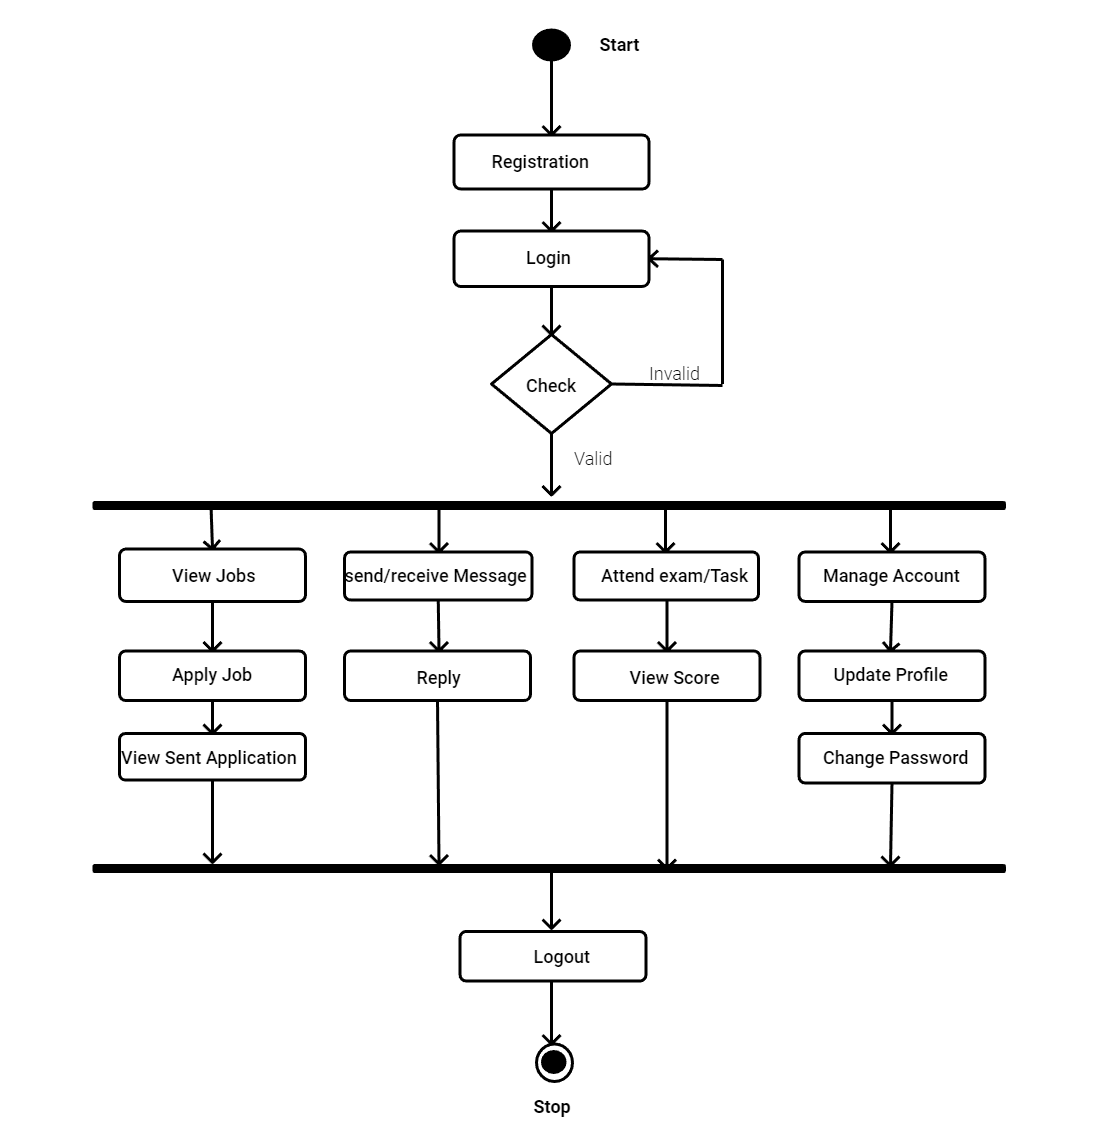
\includegraphics[width=.8\linewidth]{img/useractivity}
	\label{fig:useractivity}
    \caption{User's Activity Diagram}
\end{figure}

\pagebreak
\subitem {\centering \bf - COMPANY}
\vspace*{12pt}
\begin{figure}[bph]
	\centering
	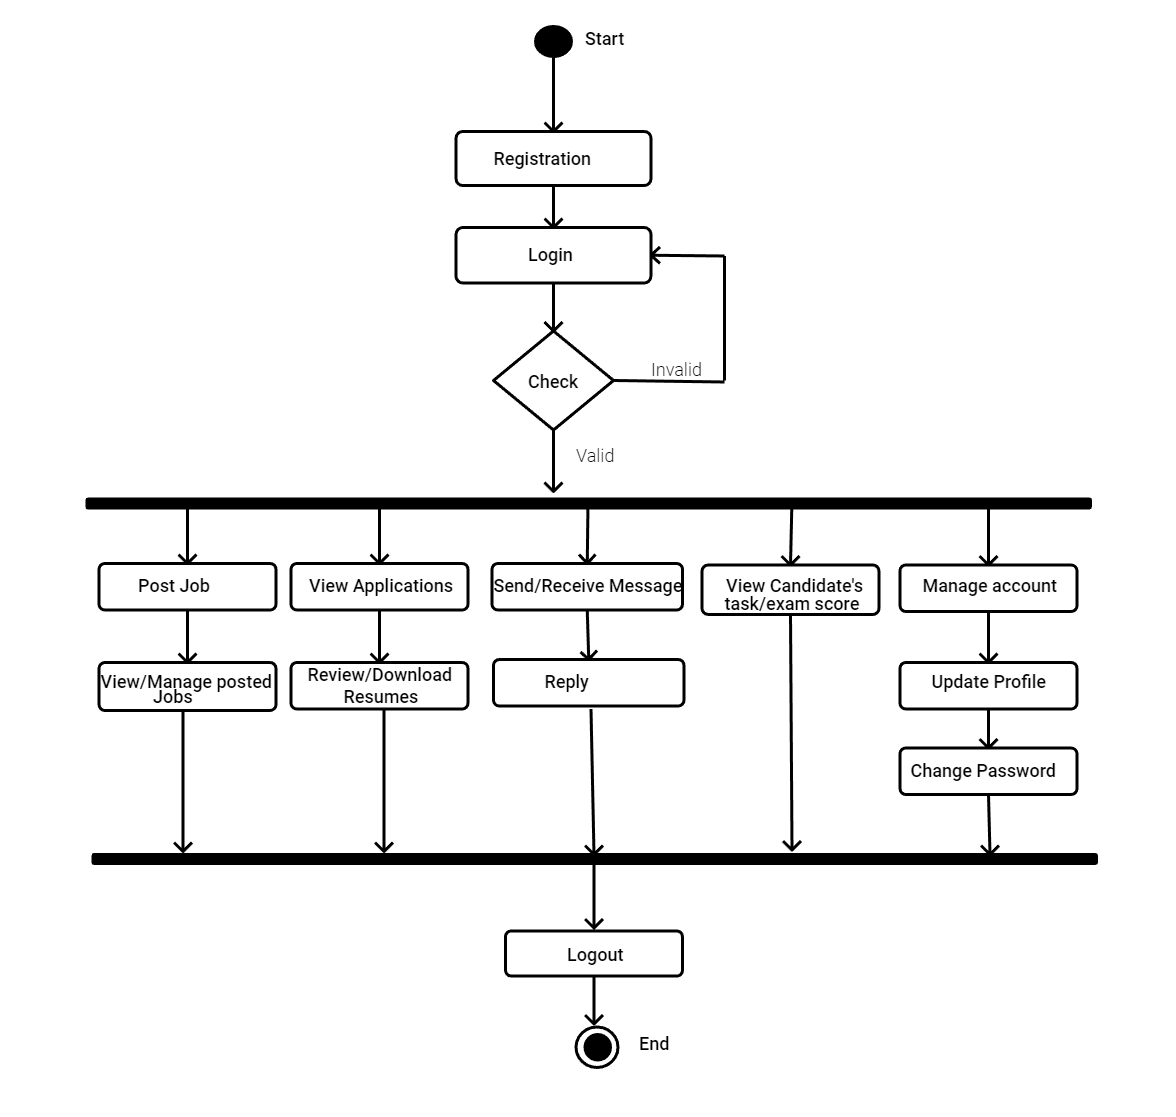
\includegraphics[width=.8\linewidth]{img/cmpnyactivity}
	\label{fig:companyactivity}
	\caption{Company's Activity Diagram}
\end{figure}

\pagebreak

\subitem {\centering \bf - ADMIN}
\vspace*{12pt}
\begin{figure}[bph]
	\centering
	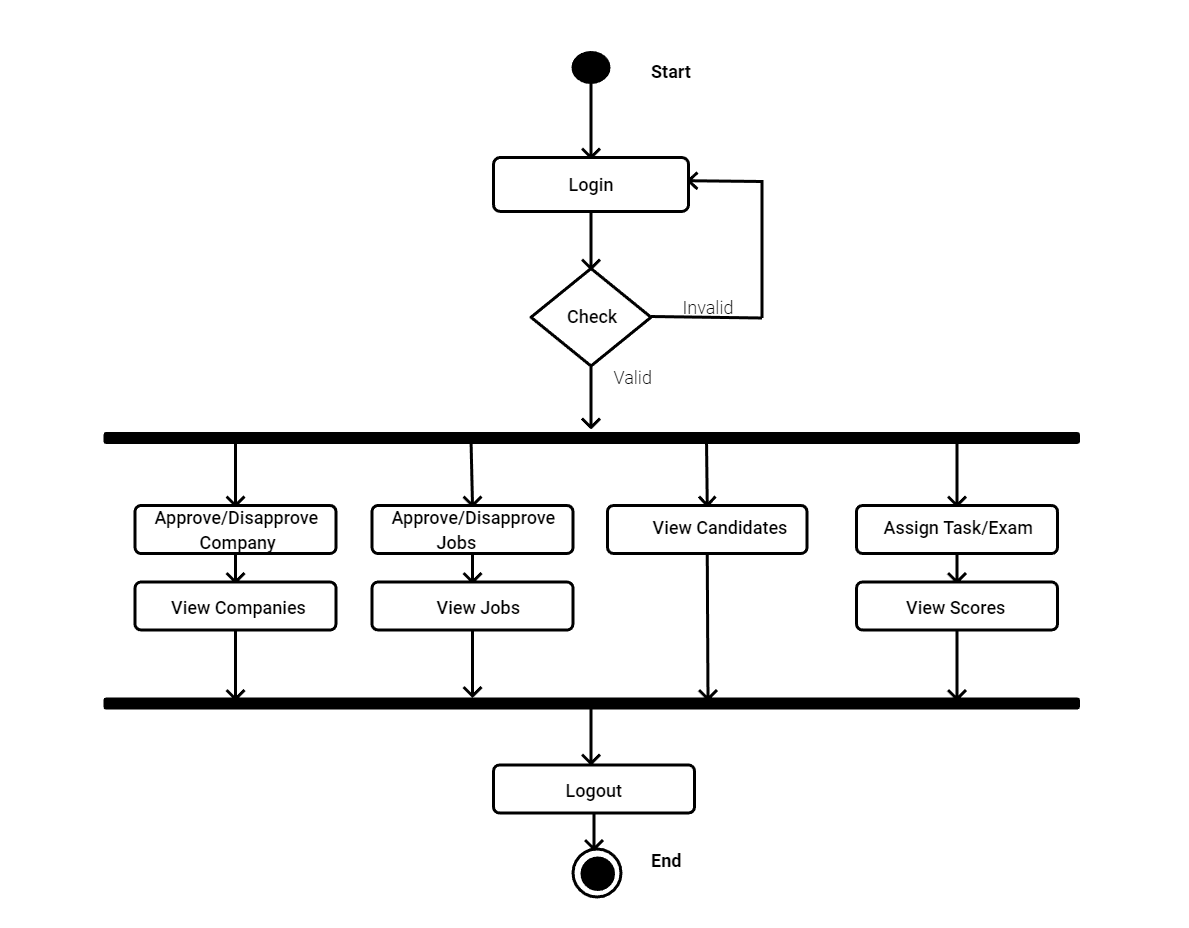
\includegraphics[width=1.1\linewidth]{img/adminactivity}
	\label{fig:adminractivity}
	\caption{Admin's Activity Diagram}
\end{figure}
\pagebreak
\subsection{UseCase Diagrams}

\vspace*{12pt}
\begin{figure}[bph]
	\centering
	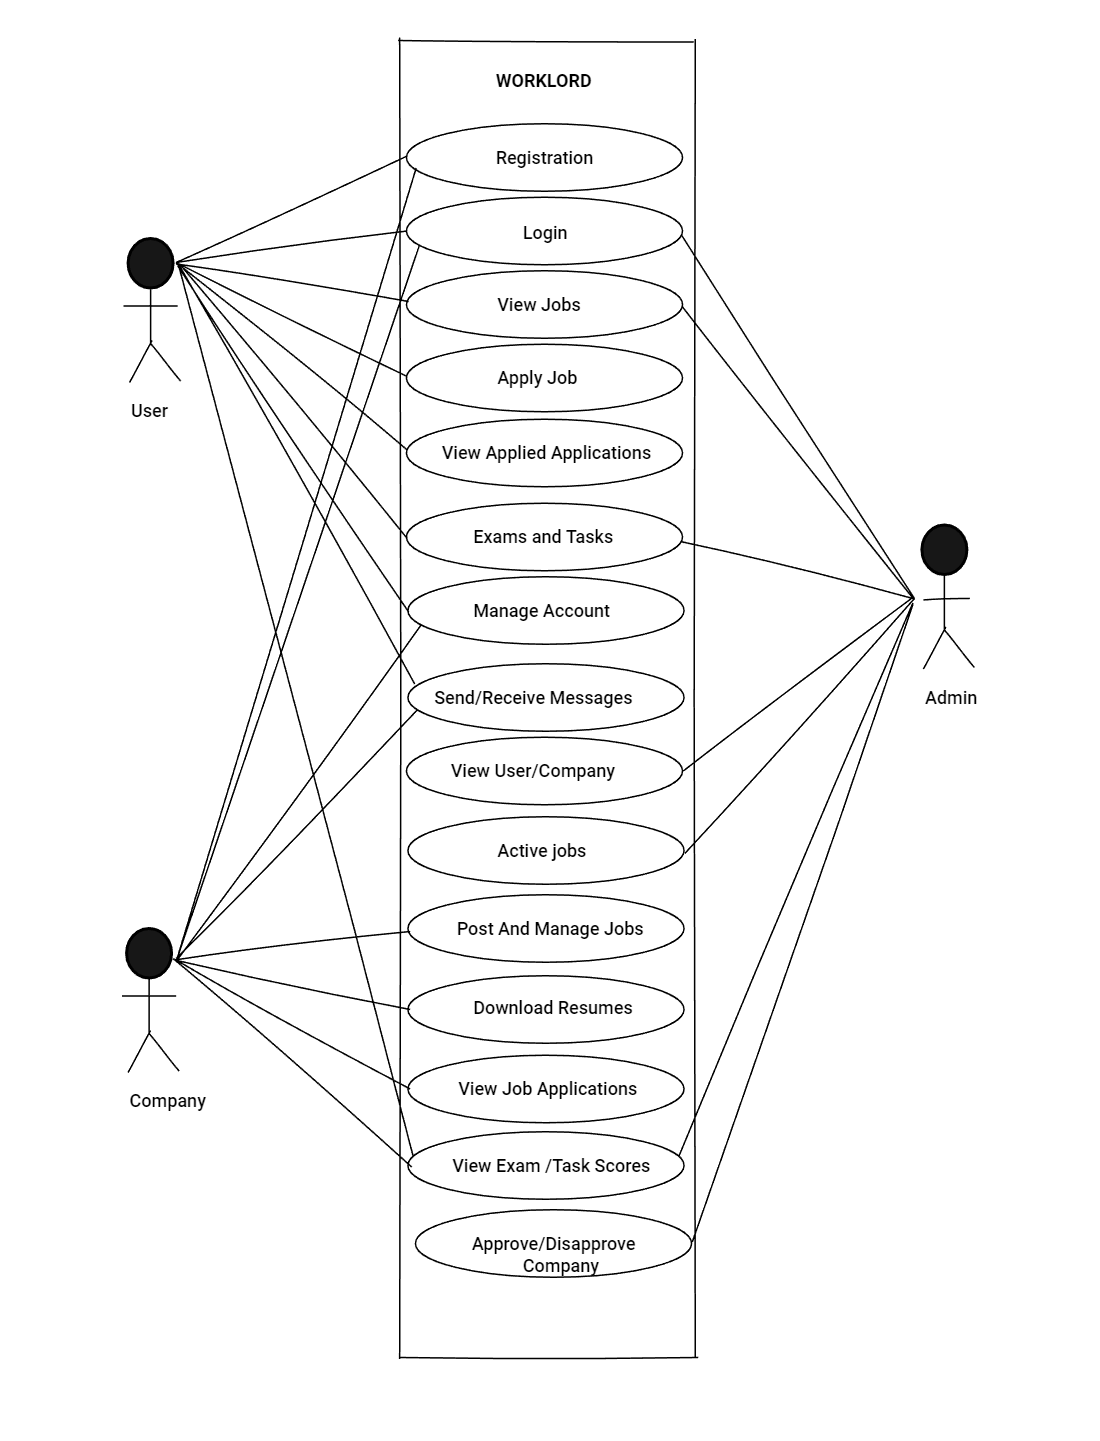
\includegraphics[width=.7\linewidth]{img/use_case_diagram}
	\label{fig:usecasediagram}
	\caption{UseCase Diagram}
\end{figure}
\pagebreak
\section{User Story}
\vspace*{12pt}

\begin{center}
	\begin{tabular}{ | p {1.5 cm} | p {4 cm} | p {3.5 cm} |  p {4.5 cm} | }
		
		\hline 
	\bf	User story ID & \bf As a $<$Type of Users$>$ & \bf I want to $<$Perform some task$>$ & \bf So that I can $<$Achieve some goal $>$ \\
		\hline
	1 & Admin/User/Company & Home Page & Go to other activities\\ \hline
	2 & User/Company & Registration & Access the system\\ \hline
	3 & Admin/User/Company & Login & Access the system\\ \hline
	4 & Admin & View companies & View companies\\ \hline
	5 & Admin & Approve,Disapprove company & Manage companies\\ \hline
	6 & Company & Post jobs & Add Job vaccancies\\ \hline
	7 & Admin & View jobs, Delete Jobs & Manage jobs\\ \hline
	8 & User & Search jobs, View jobs, Apply job, View job applications & Search jobs, View jobs, Apply job, View job applications\\ \hline
	9 & Company & View posted jobs & Manage posted jobs\\ \hline
	10 & Company & View applications, Download Resumes & View job applications, Download Resumes\\ \hline	
	11 & Admin & Create exams, Add questions & Create exams, Add questions\\ \hline
	12 & Admin & Create tasks & Create tasks\\ \hline
	13 & User & Attend exam & Attend exam\\ \hline
	14 & Admin & View candidates & View candidates\\ \hline
	15 & User & Attend task & Attend task\\ \hline
	16 & Admin/User/Company & View exam, task scores & Understand knowledge, skills of candidates\\ \hline
	17 & User/Company & Send and Receive Messages & Send/Receive Messages\\ \hline
	18 & User/Company &  Manage account & Update Profile,Change Password\\ \hline
	
	\end{tabular}
	\captionof{figure}{ User Story}
\end{center}
\pagebreak
\section{ Product Backlog}

\begin{center}
	\begin{tabular}{ | p {1.3 cm} | p {2.3 cm} | p {1 cm} |  p {1.4 cm} |  p {2.3 cm} |  p {2.0 cm} |  p {2.8 cm} | }
	
	\hline
	\centering	\bf USER STORY ID &
	\bf PRIORITY
	(LOW,HIGH,
	MEDIUM)   &
	\bf SIZE &
	\bf SPRINT & 
	\bf STATUS (PLANNED,
	PROGRESSED,
	COMPLETED) &
	\bf RELEASE DATE & 
	\bf RELEASE GOAL \\
	\hline
	
	1& HIGH & 8 & \multirow{5}{*}{1}&Completed   & 15-09-2020 &Login to the system \\ \cline{1-3} \cline{5-7} 
2& HIGH & 7 &                   &Completed   & 18-09-2020 &Access the system\\ \cline{1-3} \cline{5-7} 
3& HIGH & 8 &                   &Completed   & 20-09-2020 &Access the account\\ \cline{1-3} \cline{5-7} 
4&MEDIUM  & 8 &                   &Completed   & 23-09-2020 &View companies\\
\cline{1-3} \cline{5-7}
5& HIGH & 5 &                   &Completed   & 27-09-2020 &Manage companies \\ \cline{1-3} \cline{5-7}  \cline{1-3} \cline{5-7}
\hline
6& HIGH & 7 & \multirow{5}{*}{2}&Completed   & 30-09-2020 &Add job vaccanices\\ \cline{1-3} \cline{5-7} 
7& HIGH & 6 &                   &Completed   & 04-10-2020 &Manage jobs  \\ \cline{1-3} \cline{5-7} 

8& MEDIUM & 10 &                   &Completed   & 10-10-2020 &Search jobs,View jobs,Apply job,View job applications\\ \cline{1-3} \cline{5-7} 
9& HIGH & 6 &                   &Completed   & 11-10-2020 & Manage posted jobs\\
\cline{1-3} \cline{5-7} \hline

10& HIGH & 9 & \multirow{5}{*}{3}&Completed   & 14-10-2020 &View applications,Download Resumes \\ \cline{1-3} \cline{5-7} 
11& MEDIUM & 6 &                   &Completed   & 19-10-2020 & Create exams,Add questions \\ \cline{1-3} \cline{5-7} 
12& HIGH & 6 &                   &Completed   &22-10-2020 &Create tasks\\
\cline{1-3} \cline{5-7} 

13& MEDIUM & 6 &                   &Completed   & 26-10-2020 &Attend exams   \\ \cline{1-3} \cline{5-7}
\hline                         
\end{tabular}
\end{center}
\pagebreak

\begin{center}
	\begin{tabular}{ | p {1.3 cm} | p {2.3 cm} | p {1 cm} |  p {1.4 cm} |  p {2.3 cm} |  p {2.0 cm} |  p {2.8 cm} | }
		
		\hline
		\centering	\bf USER STORY ID &
		\bf PRIORITY
		(LOW,HIGH,
		MEDIUM)   &
		\bf SIZE &
		\bf SPRINT & 
		\bf STATUS (PLANNED,
		PROGRESSED,
		COMPLETED) &
		\bf RELEASE DATE & 
		\bf RELEASE GOAL \\
		\hline
			14& MEDIUM & 10 & \multirow{5}{*}{4}&Completed   & 28-10-2020 &View Candidates \\ \cline{1-3} \cline{5-7} 
		15&HIGH & 10 & &Completed   & 31-10-2020 &Attend task\\ \cline{1-3} \cline{5-7}
		
		16& MEDIUM & 7 &                   &Completed   & 02-11-2020 &Understand knowledge, skills of candidates\\ \cline{1-3} \cline{5-7} 
		
		17& HIGH & 8 &                   &Completed   & 05-11-2020 &Send/Receive Messages\\ \cline{1-3} \cline{5-7}
		
		18& HIGH & 8 &                   &Completed   & 08-11-2020 &Update Profile, Change password\\ \cline{1-3} \cline{5-7} \hline   
	\end{tabular}
\captionof{figure}{ Product Backlog}
\end{center}
\pagebreak
\section{Project Plan}
\vspace*{12pt}
\begin{center}
	\begin{tabular}{ | p {1.5 cm} | p {2.5 cm} | p {2 cm} |  p {2 cm} |  p {1 cm} |  p {2.2 cm} |}		
		\hline
		\centering	\bf USER STORY ID &
		\bf TASK   
		NAME     &
		\bf START
		DATE &
		\bf END
		DATE & 
		\bf DAYS &
		\bf STATUS ( TO 
		BE FILLED BY 
		SCRUM MASTER ) \\
		\hline
		
	1&\multirow{5}{*}{SPRINT 1}& 14-09-2020  & 15-09-2020  & 2 & Completed  \\ \cline{1-1} \cline{3-6}
	2&						   & 16-09-2020  & 18-09-2020  & 3 &  Completed  \\ \cline{1-1} \cline{3-6}
	3&                         & 19-09-2020  & 20-09-2020  & 2 &  Completed  \\ \cline{1-1} \cline{3-6}
	4&                         & 21-09-2020 & 23-09-2020  & 3 &  Completed  \\ \cline{1-1} \cline{3-6}
	5&                         & 24-09-2020  & 27-09-2020 & 4  &  Completed  \\ \cline{1-1} \cline{3-6}
	\hline
	
	6&\multirow{5}{*}{SPRINT 2}& 28-09-2020 & 30-09-2020  & 3 &  Completed  \\ \cline{1-1} \cline{3-6}
	7&						   & 01-10-2020  & 04-10-2020 & 4 &  Completed  \\ \cline{1-1} \cline{3-6} 
	8&						   & 05-10-2020  & 10-10-2020  & 6 &  Completed  \\ \cline{1-1} \cline{3-6}
	9&						   & 11-10-2020  & 11-10-2020  & 1 &  Completed  \\ \cline{1-1} \cline{3-6}\hline
	10&\multirow{5}{*}{SPRINT 3}&  12-10-2020 & 14-10-2020  & 3 &  Completed  \\ \cline{1-1} \cline{3-6}
	11&						   & 15-10-2020  &  19-10-2020 &5 &  Completed  \\ \cline{1-1} \cline{3-6}
	12&						   &  20-10-2020 & 22-10-2020  & 3 &  Completed  \\ \cline{1-1} \cline{3-6} 
	13&						   &  23-10-2020 & 26-10-2020  & 4 &  Completed  \\ \cline{1-1} \cline{3-6}\hline
	14&\multirow{5}{*}{SPRINT 4}&  27-10-2020 &  28-10-2020 & 2 &  Completed  \\ \cline{1-1} \cline{3-6}
	
	15&						   & 29-10-2020  & 31-10-2020  & 3 &  Completed  \\ \cline{1-1} \cline{3-6}
	16&						   & 01-11-2020  & 02-11-2020  & 2 &  Completed  \\ \cline{1-1} \cline{3-6}
	17&						   &  03-11-2020 & 05-11-2020  & 3 &  Completed  \\ \cline{1-1} \cline{3-6}
	18&						   & 06-11-2020  & 08-11-2020  & 3 &  Completed  \\ \cline{1-1} \cline{3-6}\hline
	
	
	\end{tabular}
\captionof{figure}{ Project Plan}
\end{center}
\pagebreak
\section{Sprint Backlog Planned}
\subsection {Sprint 1}
\begin{figure}[bph]
	\centering
	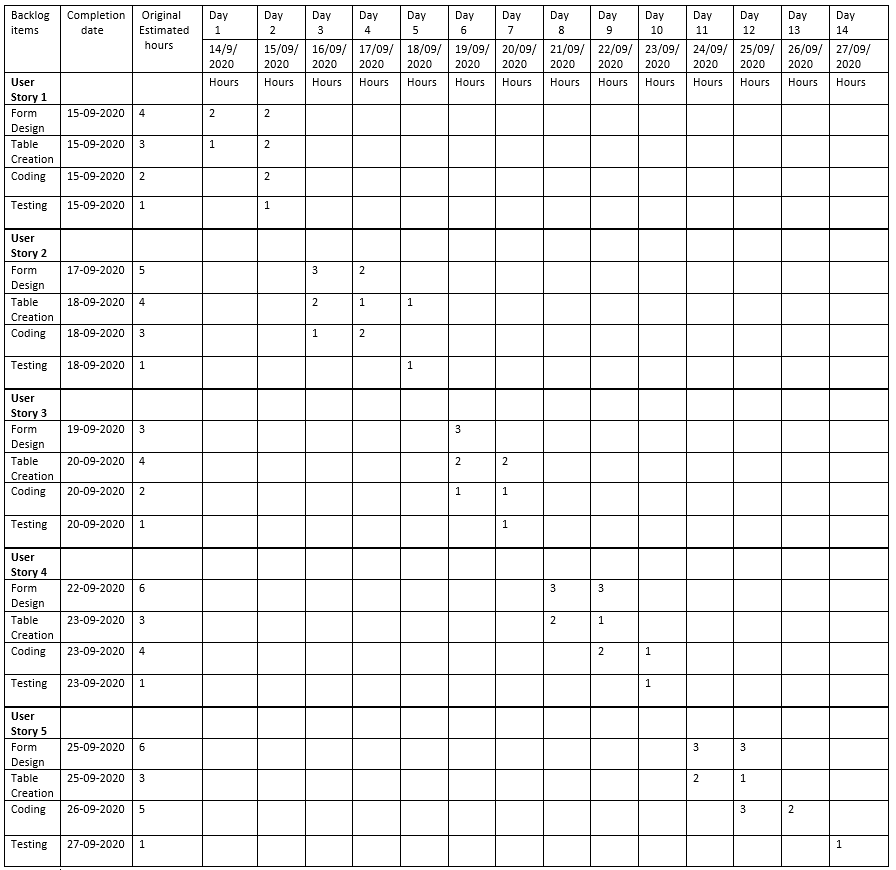
\includegraphics[width=1\linewidth]{img/sprint/sp1PLN}
	\caption{Sprint 1}
\end{figure}
\pagebreak
\subsection {Sprint 2}
\begin{figure}[bph]
	\centering
	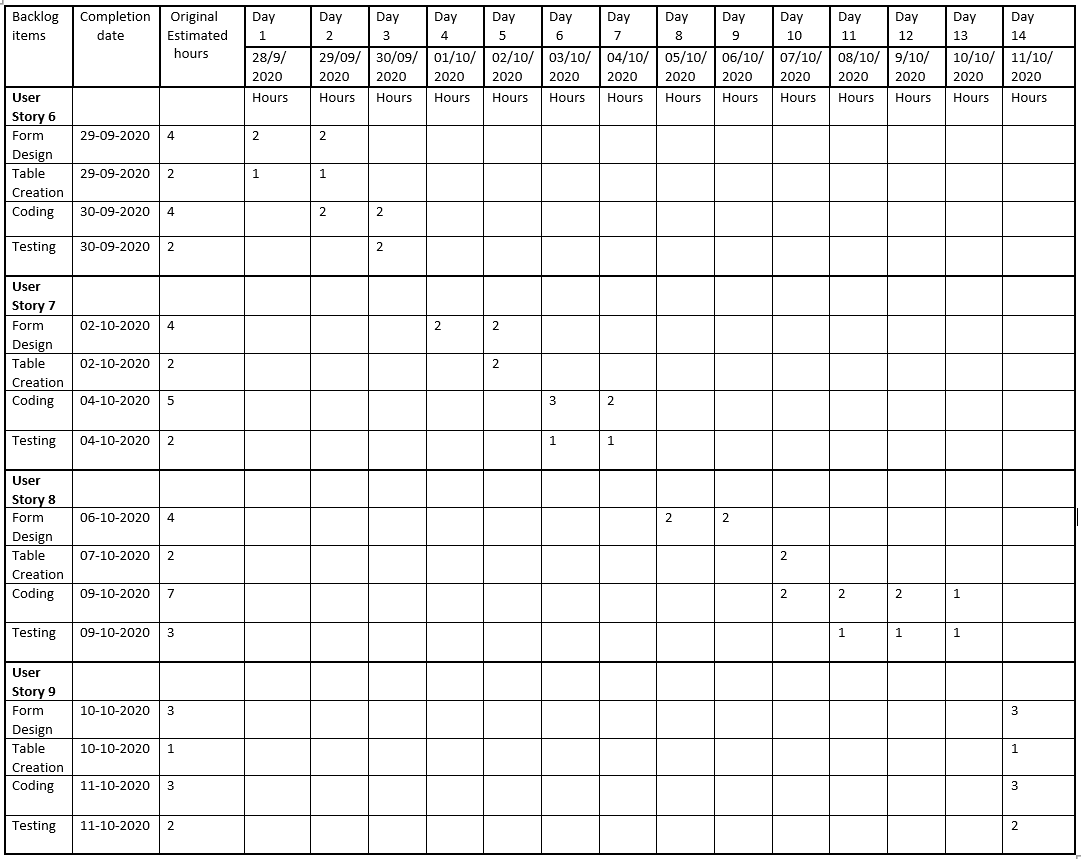
\includegraphics[width=1\linewidth]{img/sprint/SSPRINT2PLAN}
	\caption{Sprint 2}
\end{figure}
\pagebreak
\subsection {Sprint 3}
\begin{figure}[bph]
	\centering
	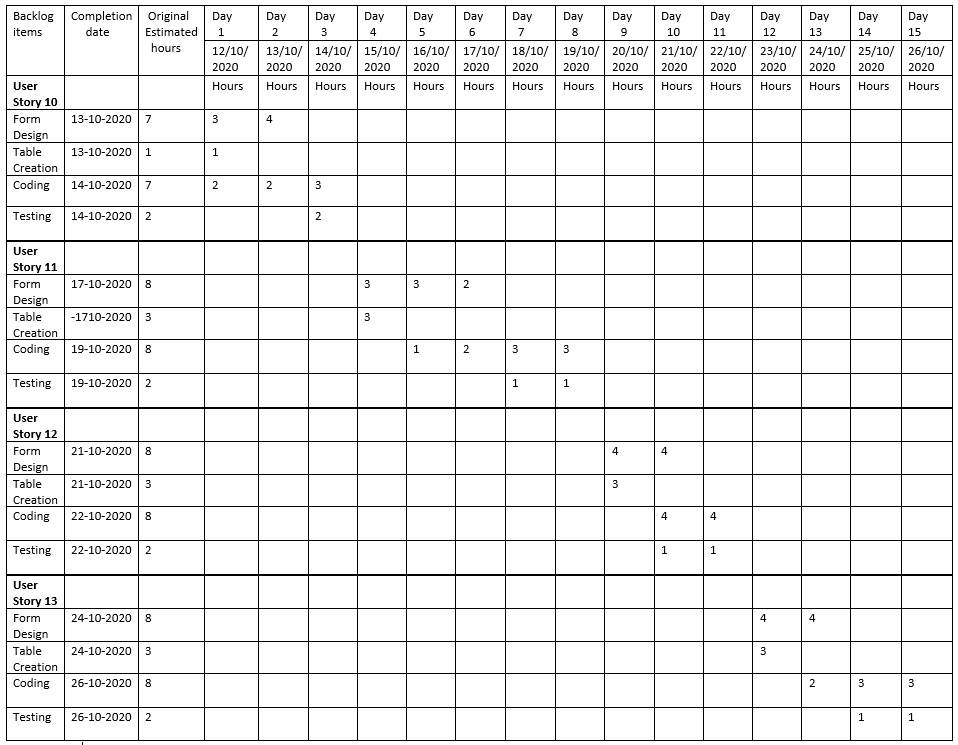
\includegraphics[width=1\linewidth]{img/sprint/sp3p}
	\caption{Sprint 3}
\end{figure}
\pagebreak
\subsection {Sprint 4}
\begin{figure}[bph]
	\centering
	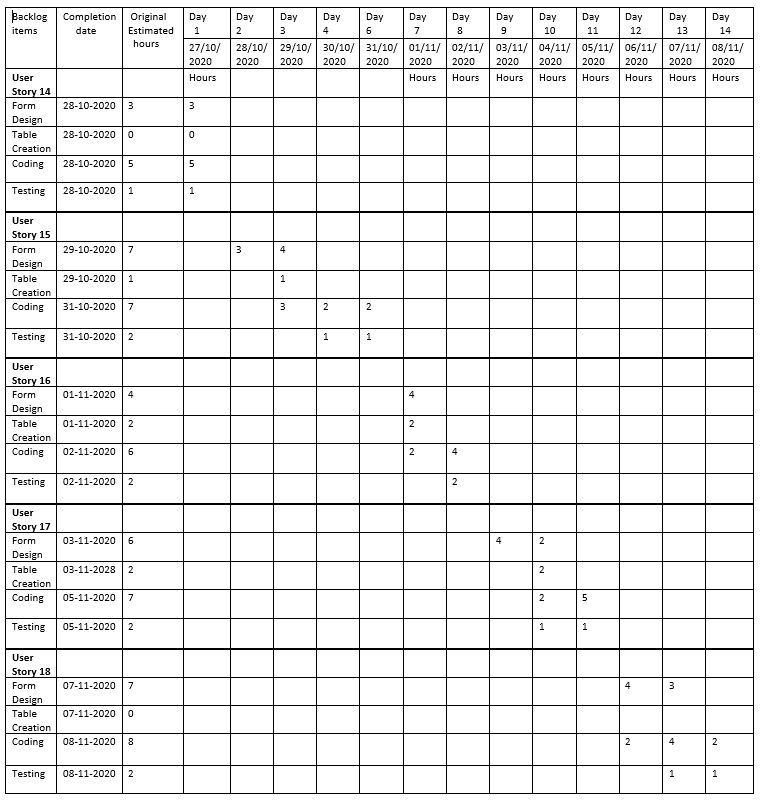
\includegraphics[width=0.9\linewidth]{img/sprint/sp4p}
	\caption{Sprint 4}
\end{figure}
\pagebreak
\section{Sprint Backlog Actual}
\subsection {Sprint 1}
\begin{figure}[bph]
	\centering
	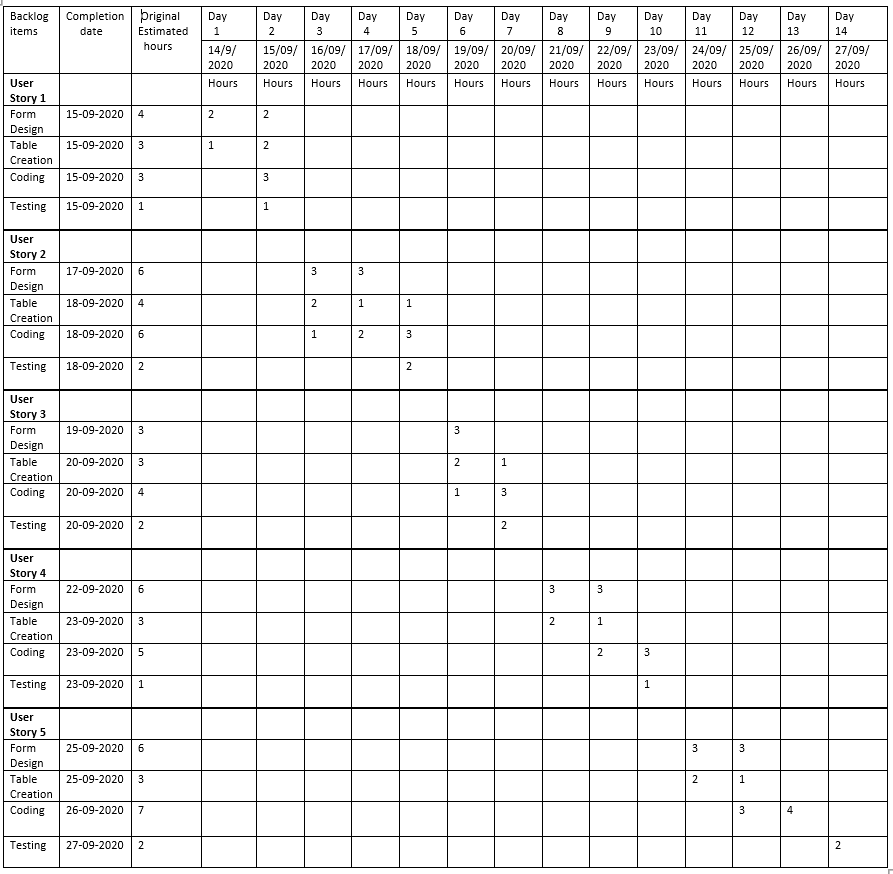
\includegraphics[width=0.9\linewidth]{img/sprint/sp1actual}
	\caption{Sprint 1}
\end{figure}
\pagebreak
\subsection {Sprint 2}
\begin{figure}[bph]
	\centering
	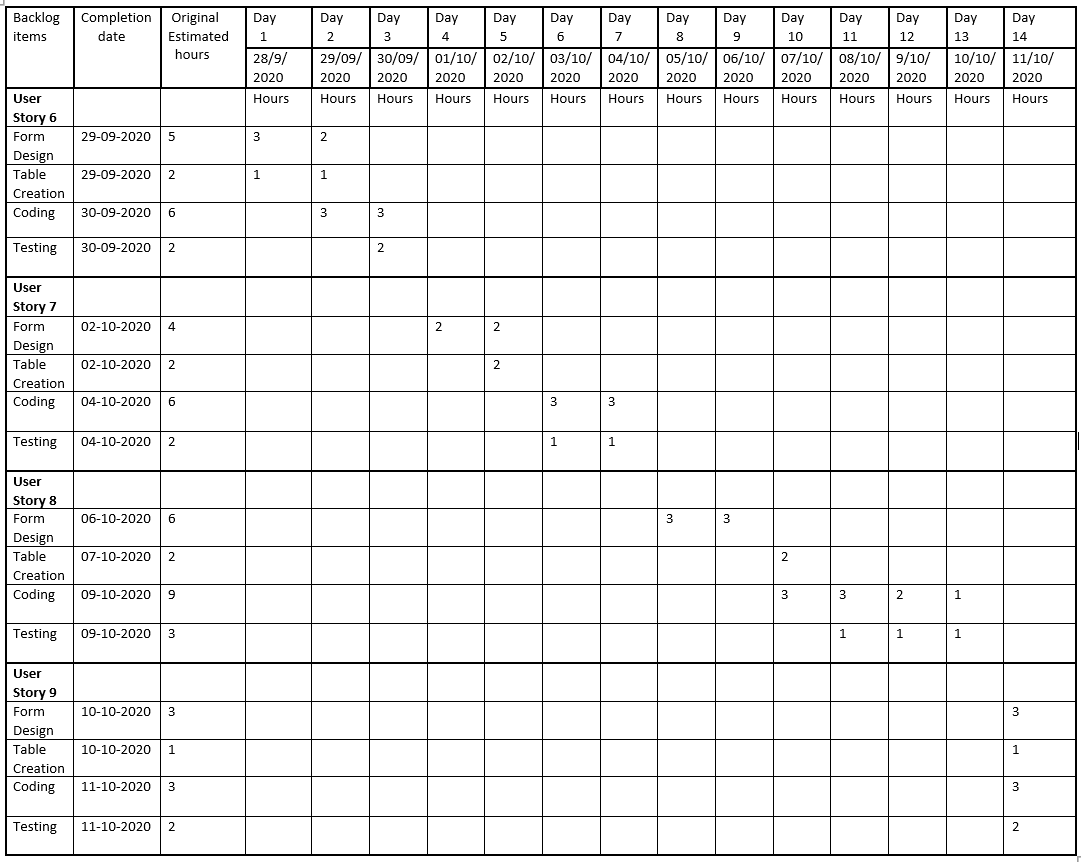
\includegraphics[width=0.9\linewidth]{img/sprint/SPRINT2ACTUAL}
	\caption{Sprint 2}
\end{figure}
\pagebreak
\subsection {Sprint 3}
\begin{figure}[bph]
	\centering
	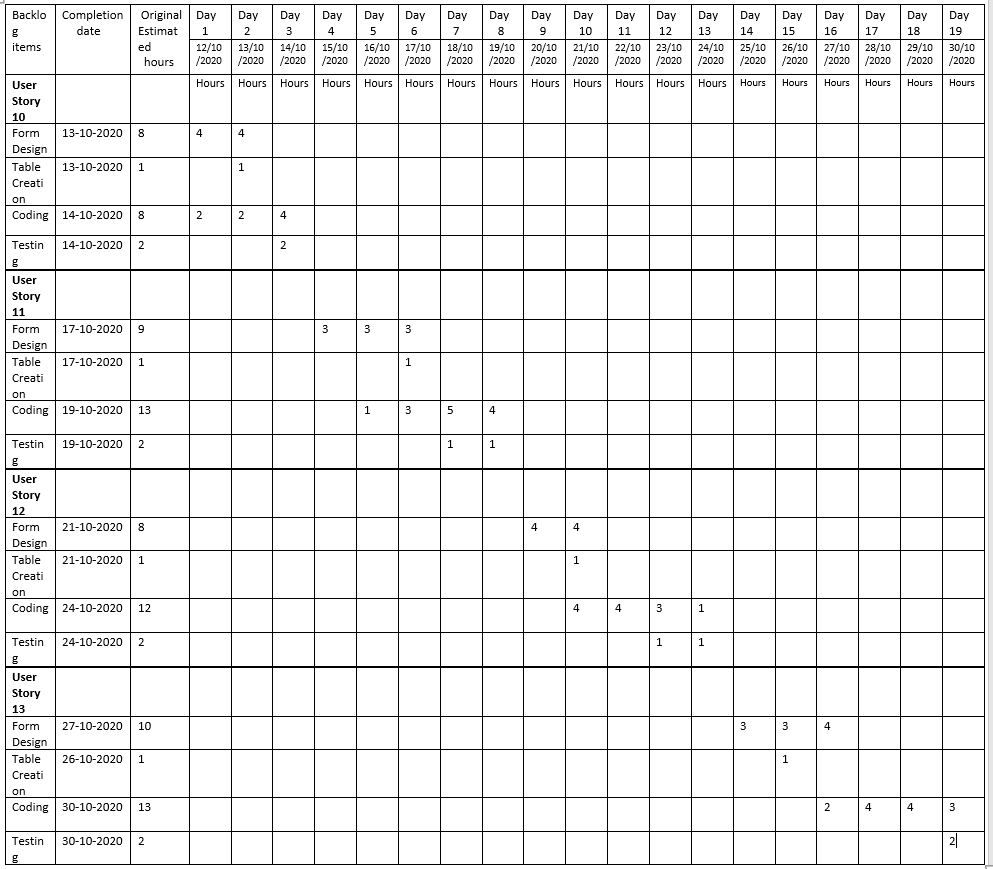
\includegraphics[width=0.9\linewidth]{img/sprint/sp3a}
	\caption{Sprint 3}
\end{figure}
\pagebreak
\subsection {Sprint 4}
\begin{figure}[bph]
	\centering
	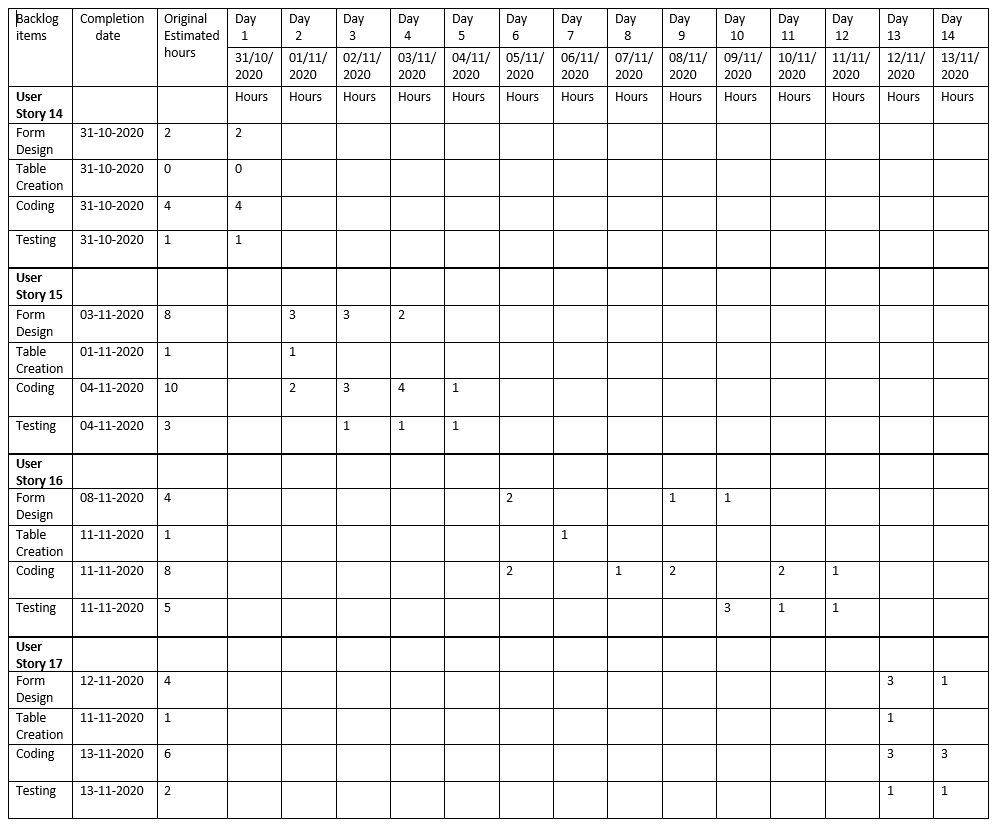
\includegraphics[width=0.9\linewidth]{img/sprint/sp4a1}
	\caption{Sprint 4}
\end{figure}
\pagebreak
\begin{figure}[bph]
	\centering
	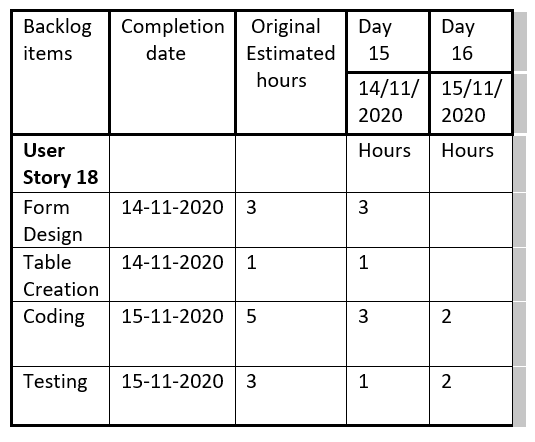
\includegraphics[width=0.5\linewidth]{img/sprint/sp4a2}
	\caption{Sprint 4}
\end{figure}
\section{Sprint Review}
\subsection {Sprint 1}
\begin{center}
	\begin{tabular}{ | p {1.5 cm} | p {5.5 cm} | p {6.0 cm} |   }
		
		\hline 
	\bf 	User story ID & \bf Comments from scrum master, if any & \bf Comments from product owner, if any \\
		\hline
		1 & Satisfied & Satisfied\\ \hline
		2 & Completed & Data enter in registration form must preserve whenever an error occure during the form validation time. \\ \hline
		3 & Satisfied  & Satisfied  \\ \hline
		4 & Satisfied  & Satisfied  \\ \hline
		5 & Satisfied & Satisfied  \\ \hline
		
	
		
	\end{tabular}
	\captionof{table}{ Sprint 1}
\end{center}
\pagebreak
\subsection {Sprint 2}

\begin{center}
	\begin{tabular}{ | p {1.5 cm} | p {5.5 cm} | p {6.0 cm} |   }
		
		\hline 
		\bf 	User story ID & \bf Comments from scrum master, if any & \bf Comments from product owner, if any \\
		\hline
		6 & Satisfied & Satisfied\\ \hline
		7 & Satisfied & Satisfied \\ \hline
		8 & Satisfied  & Satisfied  \\ \hline
		9 & Satisfied  & Satisfied  \\ \hline
		
	\end{tabular}
	\captionof{table}{ Sprint 2}
\end{center}

\subsection {Sprint 3}

\begin{center}
	\begin{tabular}{ | p {1.5 cm} | p {5.5 cm} | p {6.0 cm} |   }
		
		\hline 
		\bf 	User story ID & \bf Comments from scrum master, if any & \bf Comments from product owner, if any \\
		\hline
		10 & Satisfied & Satisfied\\ \hline
		11 & Satisfied & Satisfied \\ \hline
		12 & Satisfied  & Satisfied  \\ \hline
		13 & Completed  & Remove user id,user name and status in user view exam result.
		  \\ \hline
		
	\end{tabular}
	\captionof{table}{ Sprint 3}
\end{center}

\subsection {Sprint 4}

\begin{center}
	\begin{tabular}{ | p {1.5 cm} | p {5.5 cm} | p {6.0 cm} |   }
		
		\hline 
		\bf 	User story ID & \bf Comments from scrum master, if any & \bf Comments from product owner, if any \\
		\hline
		14 & Satisfied & Satisfied\\ \hline
		15 & Satisfied & Satisfied 	\\ \hline
		16 & Satisfied & Satisfied  \\ \hline
		17 & Satisfied & Satisfied	\\ \hline
		18 & Satisfied & Satisfied \\ \hline
	\end{tabular}
	\captionof{table}{ Sprint 4}
\end{center}

\pagebreak
\section{Database Design}
\subsection{Login Table}
Both uses and company can access their account only after login in to the system with proper username and password. This Table stores username and password of both users and company who registered in the website.

\begin{center}
	\begin{tabular} { | p {1 cm} | p {3 cm} | p {3 cm} |  p {3 cm} |  p {4 cm} | }
		
		\hline
		\centering	\bf No. &
		\bf FIELD NAME &
		\bf TYPE &
		\bf CONSTRAINTS & 
		\bf DESCRIPTION \\
		\hline
		
		
		\centering	1 &loginid & INT(3) & PRIMARY KEY & User's ID\\ \hline
		\centering	2 &email & VARCHAR(30) & UNIQUE & User's Email\\ \hline
		\centering	3 &password & VARCHAR(20) & NOTNULL &User's Password\\ \hline
		
		\centering	4 &role & VARCHAR(10) & NOTNULL &  Usertype\\ \hline
	\end{tabular}
	\vspace*{12pt}
	\captionof{table}{ Login Table}
\end{center}
\subsection{Company Table}
Any companies can gets the functionality of the system only after their registration.This Table stores Company details uploaded at the time of registration.
\begin{center}
	\begin{tabular} { | p {1 cm} | p {3.5 cm} | p {3 cm} |  p {3 cm} |  p {4 cm} | }
		
		\hline
		\centering	\bf No. &
		\bf FIELD NAME &
		\bf TYPE &
		\bf CONSTRAINTS & 
		\bf DESCRIPTION \\
		\hline
		
		1 & companyid & INT(11) & PRIMARY KEY & Company ID\\ \hline
		2 & name & VARCHAR(50) & NOTNULL & Employer's Name\\ \hline
		3 & companyname & VARCHAR(50) & NOTNULL & Company Name\\ \hline
		4 & country & VARCHAR(50) & NOTNULL & Company Country\\ \hline
		5 & state & VARCHAR(10) & NOTNULL & Company State\\ \hline
		6 & city & VARCHAR(50) & NOTNULL & Company City\\ \hline
		
		
		7 & contactno & VARCHAR(50) & NOTNULL & Company Phone Number\\ \hline
		8 & website & VARCHAR(50) & NOTNULL & Company Website\\ \hline
		9 & email & VARCHAR(50) & UNIQUE & Company's Email\\ \hline
		10 & aboutme & VARCHAR(100) & NOTNULL & About Company\\ \hline
		11 & logo & VARCHAR(100) & NOTNULL & Company Logo Name\\ \hline
		12 & active & INT(2) & NOTNULL & Account Status\\ \hline
	\end{tabular}
	
	\captionof{table}{ Company Table}
\end{center}

\pagebreak

\subsection{User Table}
Any users can gets the functionality of the system only after their registration.This Table stores details of Users uploaded at the time of registration.
\begin{center}
	\begin{tabular} { | p {1 cm} | p {3.5 cm} | p {3 cm} |  p {3 cm} |  p {4 cm} | }
		
		\hline
		\centering	\bf No. &
		\bf FIELD NAME &
		\bf TYPE &
		\bf CONSTRAINTS & 
		\bf DESCRIPTION \\
		\hline
		
		
		1 & userid & INT(11) & PRIMARY KEY & User's ID\\ \hline
		2 & firstname & VARCHAR(50) & NOTNULL & User's Firstname\\ \hline
		3 & lastname & VARCHAR(50) & NOTNULL & User's Lastname\\ \hline
		4 & email & VARCHAR(50) & UNIQUE & User's Email\\ \hline
		5 & address & VARCHAR(50) & NOTNULL & User's Address\\ \hline
		6 & country & VARCHAR(50) & NOTNULL & User's Address\\ \hline
		7 & city & VARCHAR(50) & NOTNULL & User's Country\\ \hline
		8 & state & VARCHAR(10) & NOTNULL & User's State\\ \hline
		9 & contactno & VARCHAR(50) & NOTNULL & User's Phone Number\\ \hline
		10 & qualifications & VARCHAR(50) & NOTNULL & User's Qualifications\\ \hline
		11 & stream & VARCHAR(20) & NOTNULL & User's Course\\ \hline
		12 & passingyear & VARCHAR(10) & NOTNULL & User's Year Of Passing\\ \hline
		13 & dob & DATE & NOTNULL & User's Date Of Birth\\ \hline
		14 & age & INT(3) & NOTNULL & User's Age\\ \hline
		15 & designation & VARCHAR(50) & NOTNULL & User's Preferred D6signation\\ \hline
		16 & aboutme & VARCHAR(100) & NOTNULL & About User\\ \hline
		17 & skills & VARCHAR(50) & NOTNULL & User's Skills\\ \hline
		18 & resume & VARCHAR(100) & NOTNULL & User's Resume Name\\ \hline
		
		
	\end{tabular}
	\vspace*{12pt}
	\captionof{table}{ User Table}
\end{center}
\pagebreak

\subsection{Countries Table}

This table stores the countrie's name. 
\begin{center}
	\begin{tabular} { | p {1 cm} | p {3 cm} | p {3 cm} |  p {3 cm} |  p {4 cm} | }
		
		\hline
		\centering	\bf No. &
		\bf FIELD NAME &
		\bf TYPE &
		\bf CONSTRAINTS & 
		\bf DESCRIPTION \\
		\hline
		
		
		\centering	1 &id & INT(11) & PRIMARY KEY & Country ID\\ \hline
		
		\centering	2 &name & VARCHAR(150) & UNIQUE & Country Name\\ \hline
		
		
	\end{tabular}
	\vspace*{12pt}
	\captionof{table}{ Country Table}
\end{center}
\subsection{States Table}

This table stores the names of states in each  country.
\begin{center}
	\begin{tabular} { | p {1 cm} | p {3 cm} | p {3 cm} |  p {3 cm} |  p {4 cm} | }
		
		\hline
		\centering	\bf No. &
		\bf FIELD NAME &
		\bf TYPE &
		\bf CONSTRAINTS & 
		\bf DESCRIPTION \\
		\hline
		
		
		\centering	1 &id & INT(11) & PRIMARY KEY & State ID\\ \hline
		\centering	2 &name & VARCHAR(30) & UNIQUE & State Name \\ \hline
		\centering	3 &countryid &INT(11) &FOREIGN KEY & Country ID\\ \hline
		
		
	\end{tabular}
	\vspace*{12pt}
	\captionof{table}{States Table}
\end{center}
\subsection{Cities Table}

This table stores the names of cities in each  states.
\begin{center}
	\begin{tabular} { | p {1 cm} | p {3 cm} | p {3 cm} |  p {3 cm} |  p {4 cm} | }
		
		\hline
		\centering	\bf No. &
		\bf FIELD NAME &
		\bf TYPE &
		\bf CONSTRAINTS & 
		\bf DESCRIPTION \\
		\hline
		
		
		\centering	1 &id & INT(11) & PRIMARY KEY & City ID\\ \hline
		\centering	2 &name & VARCHAR(30) & NOTNULL & City Name \\ \hline
		\centering	3 &stateid &INT(11) &FOREIGN KEY & State ID\\ \hline
		
		
	\end{tabular}
	\vspace*{12pt}
	\captionof{table}{Cities Table}
\end{center}
\pagebreak
\subsection{Job Post Table}
Each registered company can post the job vaccancies in their company.This Table stores Job Posts Details provided by the Companies
\begin{center}
	\begin{tabular} { | p {.5 cm} | p {4 cm} | p {3 cm} |  p {3 cm} |  p {4 cm} | }
		
		\hline
		\centering	\bf No. &
		\bf FIELD NAME &
		\bf TYPE &
		\bf CONSTRAINTS & 
		\bf DESCRIPTION \\
		\hline
		
		
		1 & postid & INT(3) & PRIMARY KEY & Post ID\\ \hline
		2 & companyid & INT(3) & FOREIGN KEY & Company ID\\ \hline
		3 & jobtitle & VARCHAR(20) & NOTNULL & Job Title\\ \hline
		4 & description & VARCHAR(50) & NOTNULL & About Job\\ \hline
		5 & minimumsalary & VARCHAR(20) & NOTNULL & Minimum Salary\\ \hline
		6 & maximumsalary & VARCHAR(20) & NOTNULL & Maximum Salary\\ \hline
		7 & experience & INT(3) & NOTNULL & Experience State\\ \hline
		8 & qualifications & VARCHAR(50) & NOTNULL & Job Qualifications\\ \hline
		9 & duedate & DATE & NOTNULL &Due Date \\ \hline
		
	\end{tabular}
	\vspace*{12pt}
	\captionof{table}{ Job Post Table}
\end{center}
\subsection{Job Apply Table}
Users can view the job vaccancies posted by different companies and they can apply for jobs according to their interest.This Table stores Applied User's details and status of Application
\begin{center}
	\begin{tabular} { | p {1 cm} | p {3 cm} | p {3 cm} |  p {3 cm} |  p {4 cm} | }
		
		\hline
		\centering	\bf No. &
		\bf FIELD NAME &
		\bf TYPE &
		\bf CONSTRAINTS & 
		\bf DESCRIPTION \\
		\hline
		
		1 & applyid & INT(3) & PRIMARY KEY & Job Application Apply ID\\ \hline
		2 & jobpostid & INT(3) & FOREIGN KEY & Job Post ID\\ \hline
		3 & companyid & INT(3) & FOREIGN KEY & Company ID\\ \hline
		
		4 & userid & INT(3) & FOREIGN KEY & User's ID\\ \hline
		5 & status & INT(3) & NOTNULL & Application Status\\ \hline
		
	\end{tabular}
	\vspace*{12pt}
	\captionof{table}{ Job Apply Table}
\end{center}
\pagebreak

\subsection{Exams Table}
Admin conduct exams for candidates to know their knowledge.Admin create exams and this Table stores that Exam details.
\begin{center}
	\begin{tabular} { | p {1 cm} | p {3 cm} | p {3 cm} |  p {3 cm} |  p {4 cm} | }
		
		\hline
		\centering	\bf No. &
		\bf FIELD NAME &
		\bf TYPE &
		\bf CONSTRAINTS & 
		\bf DESCRIPTION \\
		\hline
		
		1 & examid & INT(3) & PRIMARY KEY & Exam ID\\ \hline
	
		2 & examname & VARCHAR(30) & NOTNULL & Exam Name\\ \hline
		3 & duration & INT(3) & NOTNULL & Exam Duration\\ \hline
		4 & passmark & INT(5) & NOTNULL & Exam Passmark\\ \hline
	
		5 & terms & VARCHAR(150) & NOTNULL & Exam Terms\\ \hline	
		
	\end{tabular}
	\vspace*{12pt}
	\captionof{table}{ Exams Table}
\end{center}

\subsection{Exam Questions Table}
Admin conduct exams for candidates to know their knowledge,so admin need to be add and upadate questions.This table stores the questions for each exams.
\begin{center}
	\begin{tabular} { | p {1 cm} | p {3 cm} | p {3 cm} |  p {3 cm} |  p {4 cm} | }
		
		\hline
		\centering	\bf No. &
		\bf FIELD NAME &
		\bf TYPE &
		\bf CONSTRAINTS & 
		\bf DESCRIPTION \\
		\hline
		
		
		1 & questionid & INT(3) & PRIMARY KEY & Question ID\\ \hline
		2 & examid & VARCHAR(15) & FOREIGN KEY & Exam ID\\ \hline
		3 & type & VARCHAR(50) & NOTNULL & Question Category\\ \hline
		4 & question & LONGTEXT & NOTNULL & Question \\ \hline
		5 & option1 & VARCHAR(50) & NOTNULL & Question Option 1\\ \hline 
		6 & option2 & VARCHAR(50) & NOTNULL &Question Option 2 \\ \hline
		7 & option3 & VARCHAR(50) & NOTNULL & Question Option 3 \\ \hline
		8 & option4 & VARCHAR(50) & NOTNULL & Question Option 4 \\ \hline
		9 & answer & VARCHAR(50) & NOTNULL & Question Answer  \\ \hline
		
	\end{tabular}
	\vspace*{12pt}
	\captionof{table}{ Exam Questions Table}
\end{center}


\pagebreak

\subsection{Assessment Record Table}
Each candidates should attend the exam assigned by the admin and the exam score can be view by the admin,company and user.This table store
exam scores of each candidates.
\begin{center}
	\begin{tabular} { | p {1 cm} | p {3 cm} | p {3 cm} |  p {3 cm} |  p {4 cm} | }
		
		\hline
		\centering	\bf No. &
		\bf FIELD NAME &
		\bf TYPE &
		\bf CONSTRAINTS & 
		\bf DESCRIPTION \\
		\hline
		
		
		1 & recordid & INT(3) & PRIMARY KEY & Record ID\\ \hline
		2 & userid & INT(3) & FOREIGN KEY & User's ID\\ \hline
		3 & examid & VARCHAR(20) & FOREIGN KEY & Exam ID\\ \hline
		4 & score &INT(5) & NOTNULL & User's Score\\ \hline
		5 & status &INT(2) & NOTNULL & Result Status\\ \hline
		6 & date & DATE & NOTNULL & Exam Date\\ \hline
		
		
	\end{tabular}
	\captionof{table}{ Assessment Record  Table}
\end{center}
\subsection{Task Table}
Admin assign different tasks for candidates to know their skills. This table store task details that assigned by admin for candidates.
\begin{center}
	\begin{tabular} { | p {1 cm} | p {3 cm} | p {3 cm} |  p {3 cm} |  p {4 cm} | }
		
		\hline
		\centering	\bf No. &
		\bf FIELD NAME &
		\bf TYPE &
		\bf CONSTRAINTS & 
		\bf DESCRIPTION \\
		\hline
		
		1 & taskid & INT(3) & PRIMARY KEY & Task ID\\ \hline
			2 & taskname & VARCHAR(50) & NOTNULL & Task Name\\ \hline
		3 & question & VARCHAR(500) & NOTNULL & Question\\ \hline
		4 & passmark & INT(3)) & NOTNULL & Pass Mark\\ \hline
		5 & terms & LONGTEXT & NOTNULL & Task Details\\ \hline
		6 & status & INT(2)	 & NOTNULL & Task Status\\ \hline
	\end{tabular}
	\captionof{table}{ Task Table}
\end{center} 
\pagebreak
\subsection{Task Submit Table}
Each candidate responsible for complete the task assigned for them.This table stores candidates's submitted task details,status and scores.

\begin{center}
	\begin{tabular}[ht] { | p {1 cm} | p {3 cm} | p {3 cm} |  p {3 cm} |  p {4 cm} | }
		
		\hline
		\centering	\bf No. &
		\bf FIELD NAME &
		\bf TYPE &
		\bf CONSTRAINTS & 
		\bf DESCRIPTION \\
		\hline
		
		1 & taskid & INT(3) & PRIMARY KEY & Task ID\\ \hline
		2 & userid & INT(3) & FOREIGN KEY & Candidate ID\\ \hline
		3 & tasksubmitdate & DATE & NOTNULL & Task Submit Date\\ \hline
		4 & tasksubmitstatus & INT(5) & NOTNULL & Task Submit Status\\ \hline
		5 & taskreviewstatus & INT(5) & NOTNULL & Task Review Status\\ \hline
		6 & tasklink & VARCHAR(200) & NOTNULL & Task Github Link\\ \hline
		7 & taskscore & INT(10) & NOTNULL & Task Status\\ \hline
		
	\end{tabular}
	\captionof{table}{ Tasks Submit Table}
\end{center}


\subsection{MailBox}
There is an option to make communication between user and company.This Table stores Mail details that is to be send/receive from user/company.

\begin{center}
	\begin{tabular}[ht] { | p {1 cm} | p {3 cm} | p {3 cm} |  p {3 cm} |  p {4 cm} | }
		
		\hline
		\centering	\bf No. &
		\bf FIELD NAME &
		\bf TYPE &
		\bf CONSTRAINTS & 
		\bf DESCRIPTION \\
		\hline
		
		1 & idmailbox & INT(3) & PRIMARY KEY & Mail ID\\ \hline
		2 & idfromuser & INT(3) & NOTNULL & ID of user send message\\ \hline
		3 & fromuser & VARCHAR(10) & NOTNULL & Type of user who send\\ \hline
		4 & idtouser & INT(3) & NOTNULL & The id of user to be send\\ \hline
		5 & subject & VARCHAR(100) & NOTNULL & Message subject\\ \hline
		6 & message & VARCHAR(300) & NOTNULL & Message \\ \hline
		7 & date & DATE & NOTNULL & Date of message creation\\ \hline
		
	\end{tabular}
	\captionof{table}{ MailBox Table}
\end{center}
\pagebreak
\subsection{Reply MailBox}
There is an option to make communication between user and company.This Table stores Mail details that is to be send/receive from user/company.

\begin{center}
	\begin{tabular}[ht] { | p {1 cm} | p {3 cm} | p {3 cm} |  p {3 cm} |  p {4 cm} | }
		
		\hline
		\centering	\bf No. &
		\bf FIELD NAME &
		\bf TYPE &
		\bf CONSTRAINTS & 
		\bf DESCRIPTION \\
		\hline
			1 & idreply & INT(3) &  PRIMARY KEY   & ID of reply message\\ \hline
		2 & idmailbox & INT(3) & FOREIGN KEY  & Mail ID\\ \hline
	
		3 & iduser & VARCHAR(10) & FOREIGN KEY & ID of user \\ \hline
		4 & usertype & INT(3) & FOREIGN KEY & Type of user\\ \hline
	
		6 & message & VARCHAR(300) & NOTNULL & Message \\ \hline
		7 & date & DATE & NOTNULL & Date of message creation\\ \hline
		
	\end{tabular}
	\captionof{table}{Reply MailBox Table}
\end{center}



\pagebreak
\section{User Interface Design}
\subsection {Homepage}
This form show Homepage of Worklord Website.From which we can go to all other activities.
\begin{figure}[bph]
	\centering
	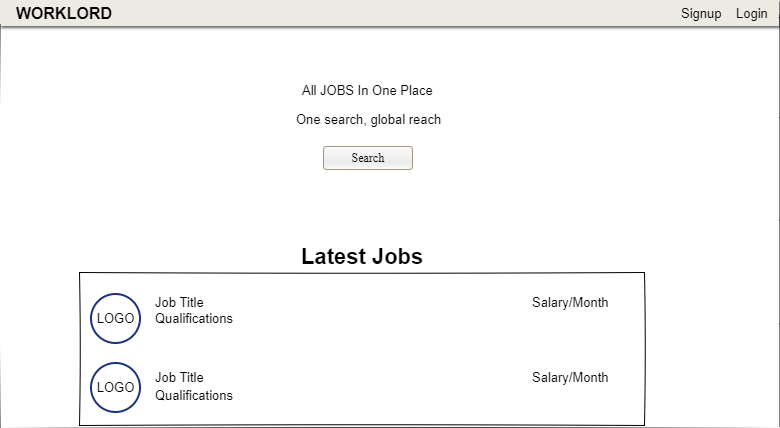
\includegraphics[width=.4\linewidth]{img/homepage}
	\caption{Homepage}
\end{figure}
\subsection {Login}
Once registerd in the website,using this Page admin,company and users can login to their accounts.
\begin{figure}[bph]
	\centering
	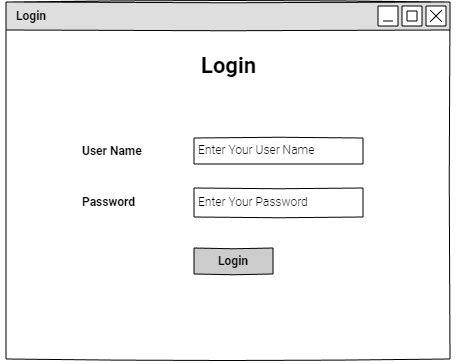
\includegraphics[width=.4\linewidth]{img/login}
	\caption{Login}
\end{figure}
\pagebreak

\subsection {Job Search}
Helps to Search Available Jobs in the website.There is also an option to searrch jobs based on experience,job name etc.
\begin{figure}[bph]
	\centering
	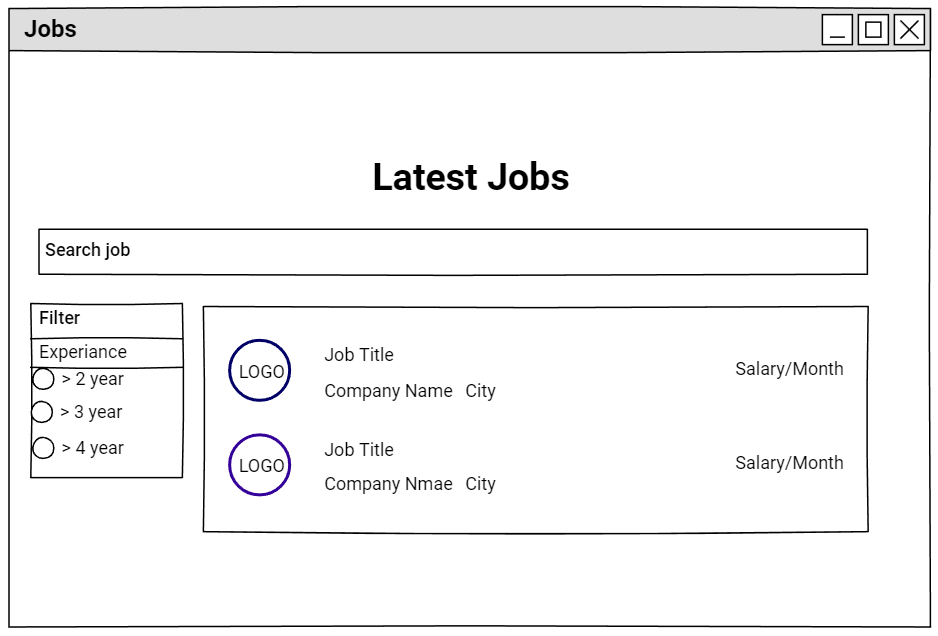
\includegraphics[width=.65\linewidth]{img/usersearchjob}
	\caption{Job Search}
\end{figure}
\subsection {Jobs}
Show the each of the job Details.and also candidate can apply for particular job.
\begin{figure}[bph]
	\centering
	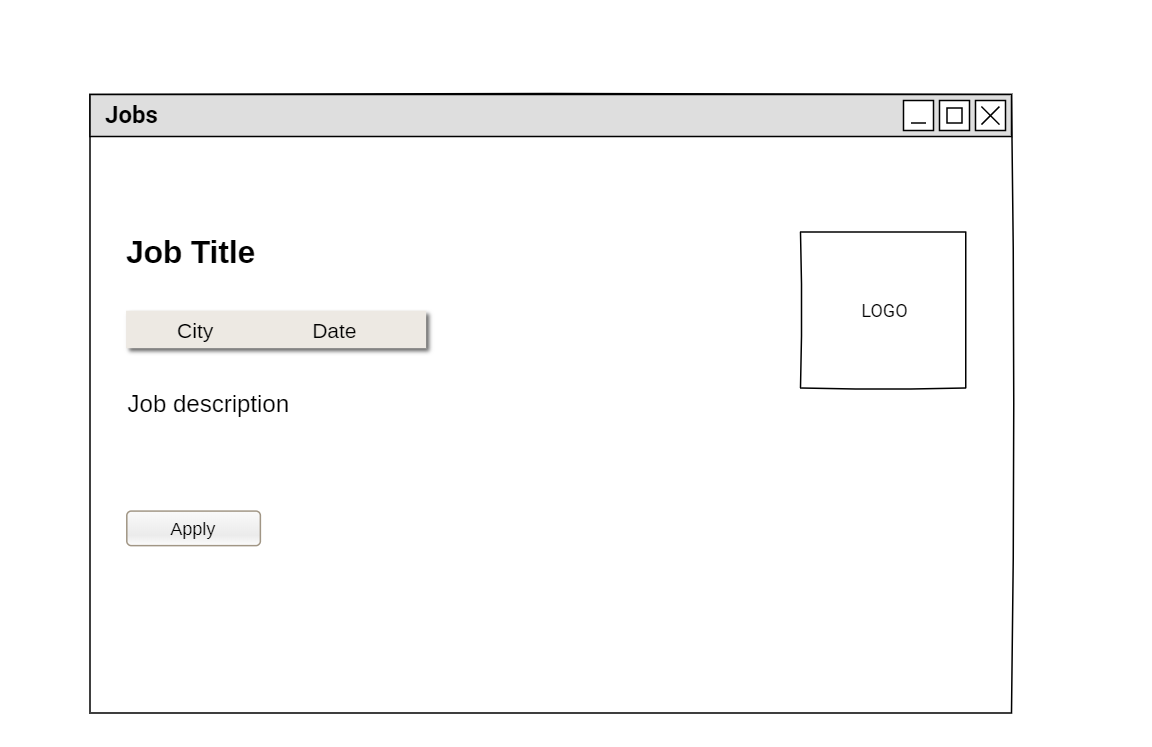
\includegraphics[width=.6\linewidth]{img/user/userappyjob}
	\caption{Jobs}
\end{figure}
\pagebreak

\subsection {Mailbox}
View messages from User/Company and Compose messages to User/Company
\begin{figure}[bph]
	\centering
	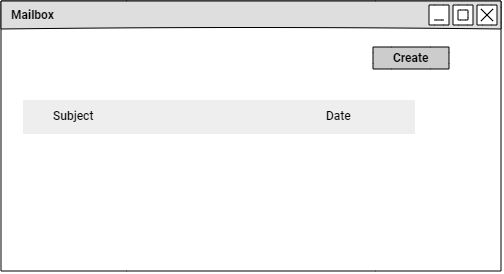
\includegraphics[width=.7\linewidth]{img/notification}
	\caption{MailBox}
\end{figure}


\subsection {View Mailbox}
View messages from User/Company and Reply to those messages
\begin{figure}[bph]
	\centering
	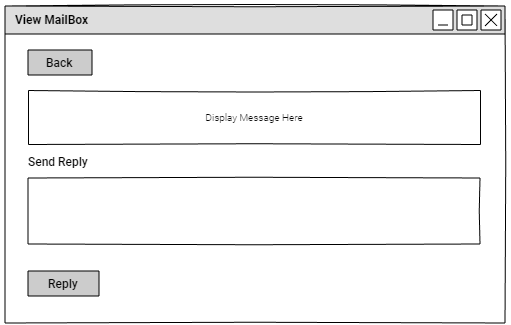
\includegraphics[width=.7\linewidth]{img/view_notifctn}
	\caption{View MailBox}
\end{figure}
\pagebreak

\subsection {Compose Message}
Compose Messages to User or Company (Shows users Applied for Jobs)
\begin{figure}[bph]
	\centering
	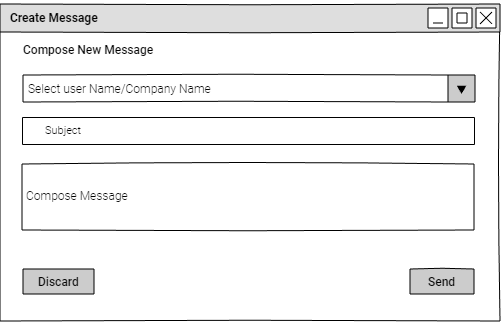
\includegraphics[width=.5\linewidth]{img/create_msg}
	\caption{Compose Message}
\end{figure}
\addcontentsline{toc}{section}{ - User}
\subsection {User Registration}
Registration form for User
\begin{figure}[bph]
	\centering
	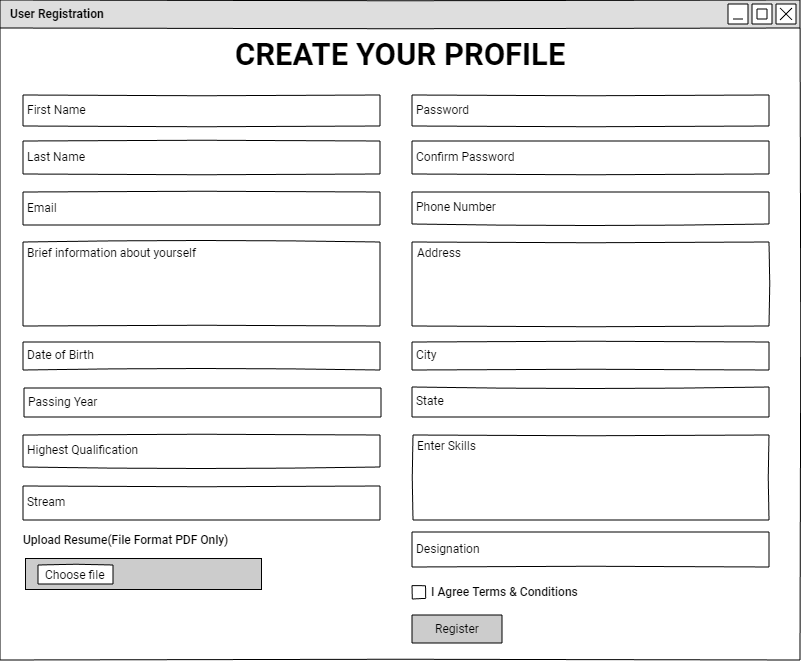
\includegraphics[width=.6\linewidth ]{img/user/user_registration}
	\caption{User Registration}
\end{figure}
\pagebreak

\subsection { User Dashboard}
Dashboard for Users, Shows available functions for user
\begin{figure}[bph]
	\centering
	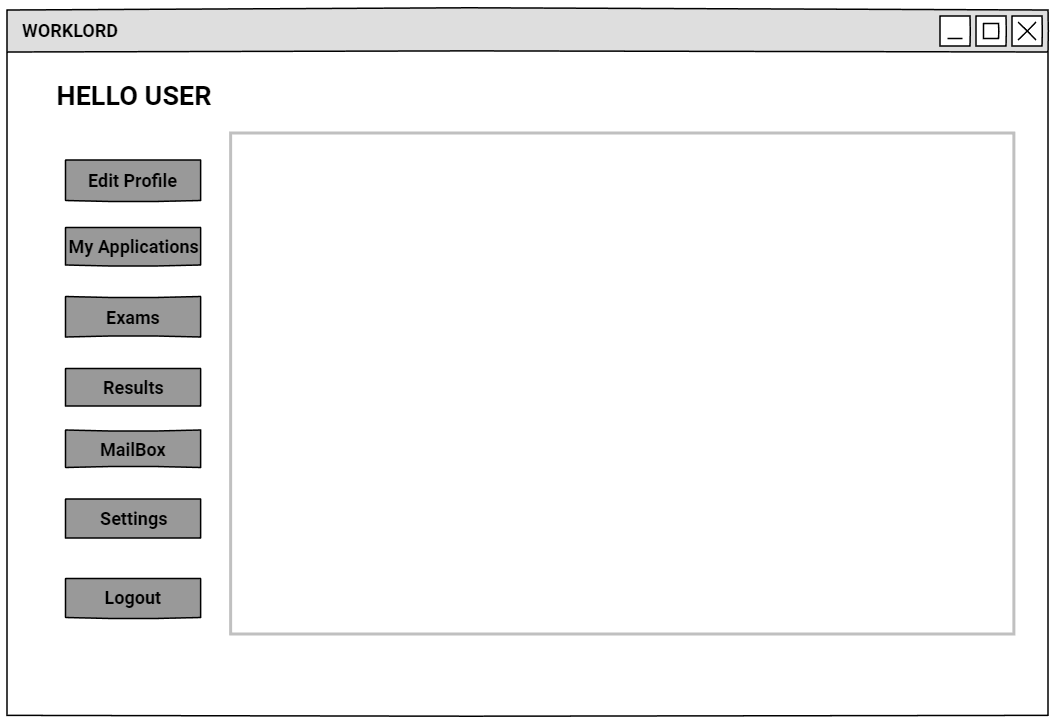
\includegraphics[width=.8\linewidth]{img/user/userhme}
	\caption{User Dashboard}
\end{figure}
\pagebreak
\subsection {My Applications}
This show Applied Job's Details and Status
\begin{figure}[bph]
	\centering
	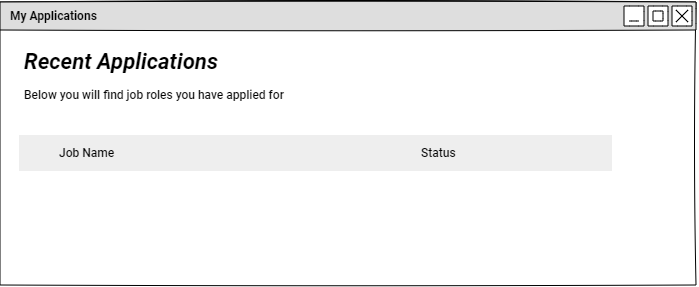
\includegraphics[width=.7\linewidth]{img/user/useraplictns}
	\caption{My Applications}
\end{figure}

\subsection {Update Profile}
Update User's Details and Resume.
\begin{figure}[bph]
	\centering
	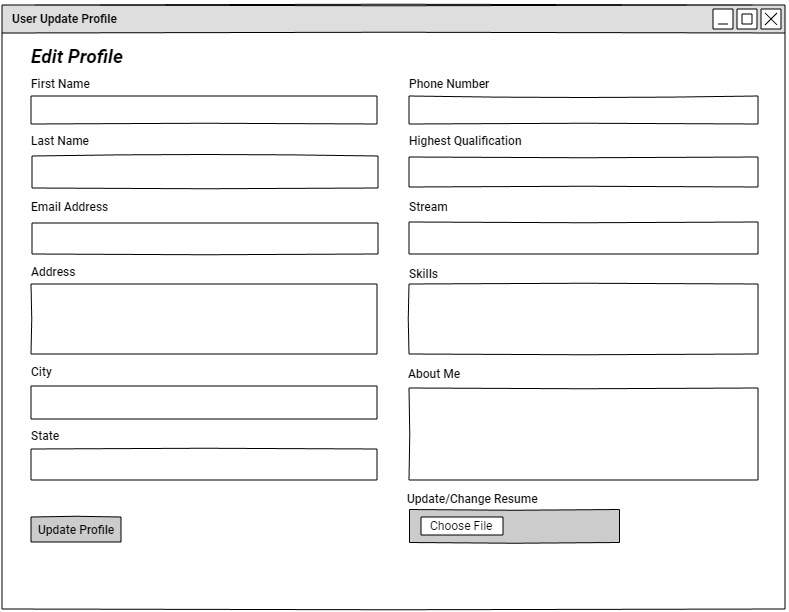
\includegraphics[width=.7\linewidth ]{img/user/userupdate}
	\caption{Update Profile}
\end{figure}

\subsection {User Exam Overview}
Attend Exams and View scores
\begin{figure}[bph]
	\centering
	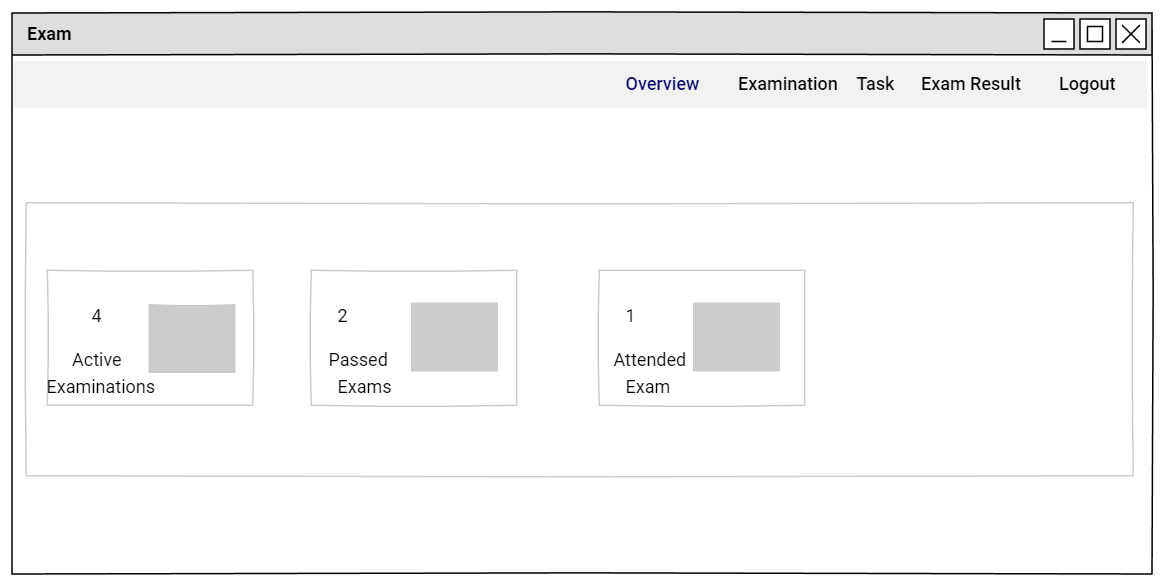
\includegraphics[width=.4\linewidth]{img/user/userexamoverview}
		\caption{User Exam Overview}
\end{figure}
\subsection {User view Examlist}
Attend Exams and View scores
\begin{figure}[bph]
	\centering
	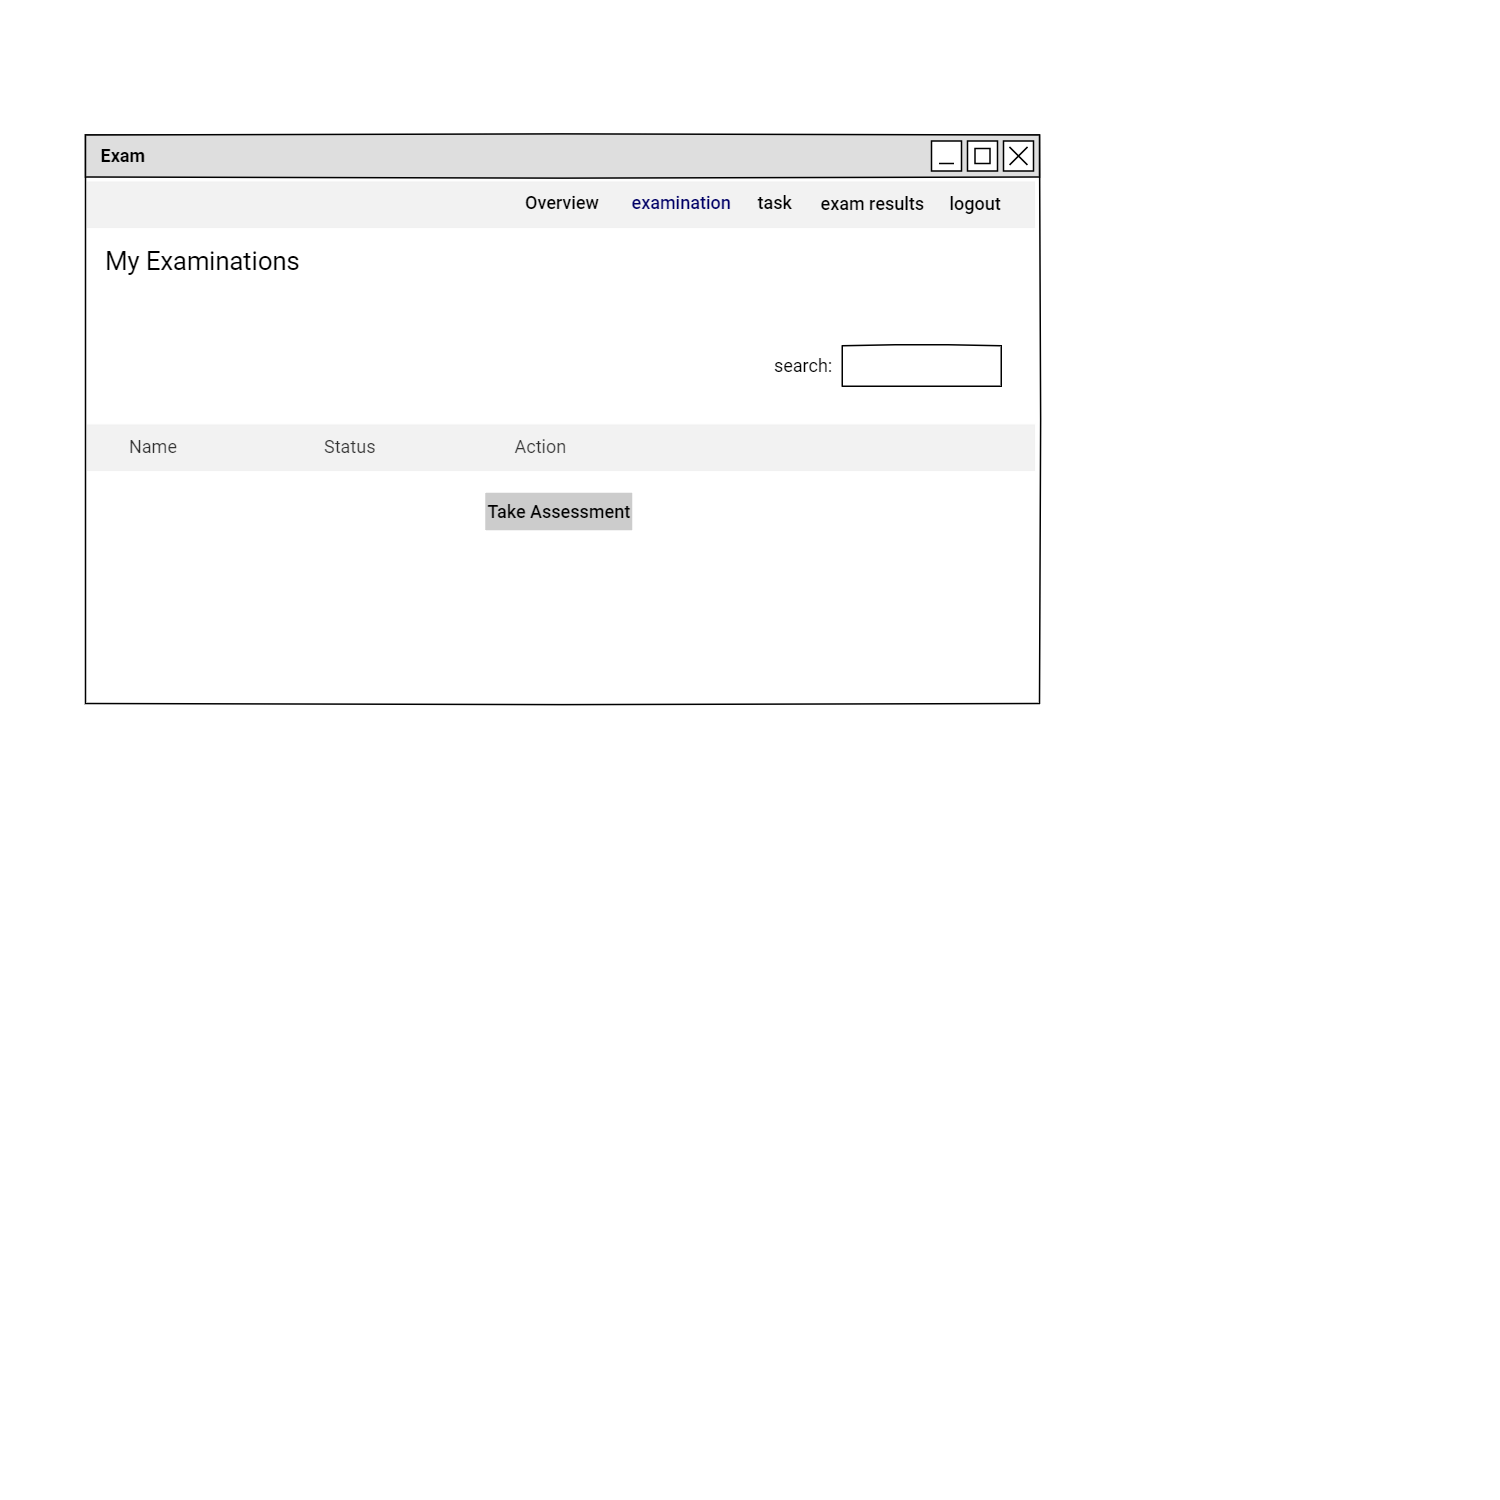
\includegraphics[width=.4\linewidth]{img/user/useviewexamlist}
	\caption{User view Examlist}
	\end{figure}
\pagebreak
\subsection {User Take Assessment}
Attend Exams and View scores
\begin{figure}[bph]
	\centering
	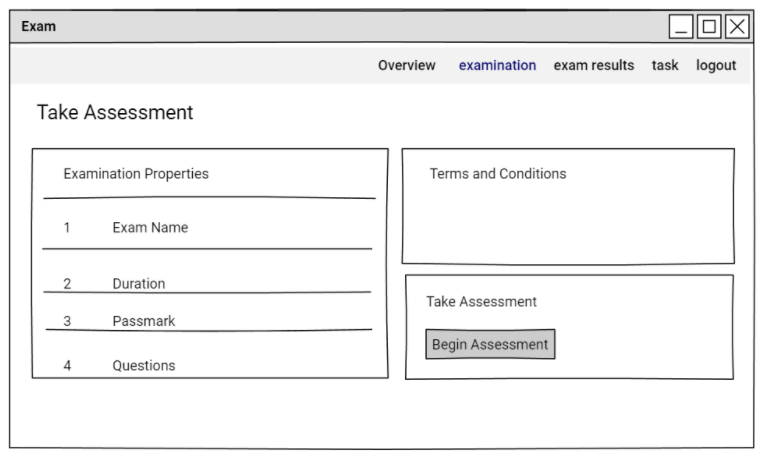
\includegraphics[width=.4\linewidth]{img/user/examassessmnt}
	\caption{ User Take Assessment}
\end{figure}
\subsection {User Attend Exam}
Attend Exams and View scores
\begin{figure}[bph]
	\centering
	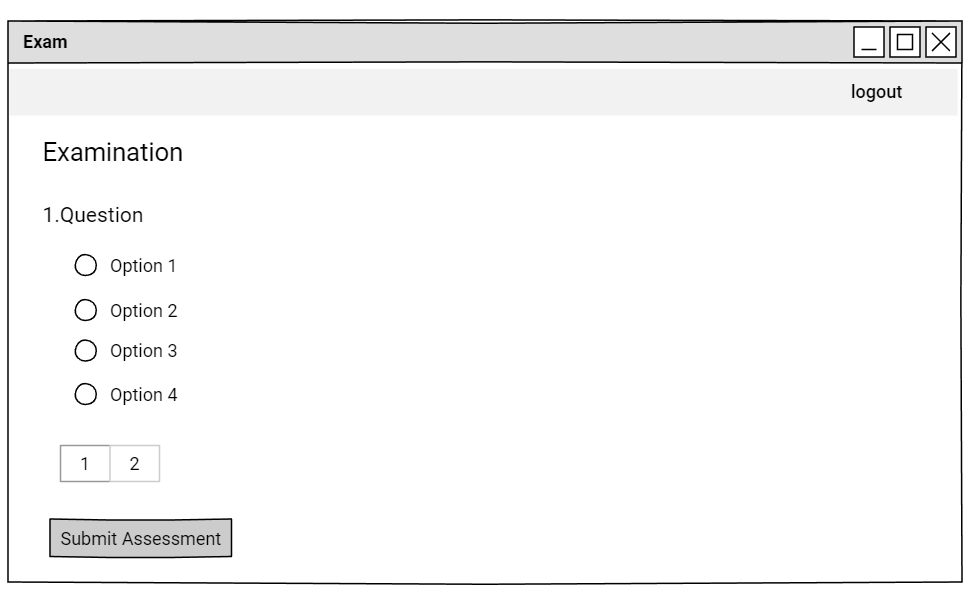
\includegraphics[width=.4\linewidth]{img/user/attendexam}
	\caption{User Attend Exam}
\end{figure}
\pagebreak
\subsection {User View Tasks}
Attend Tasks
\begin{figure}[bph]
	\centering
	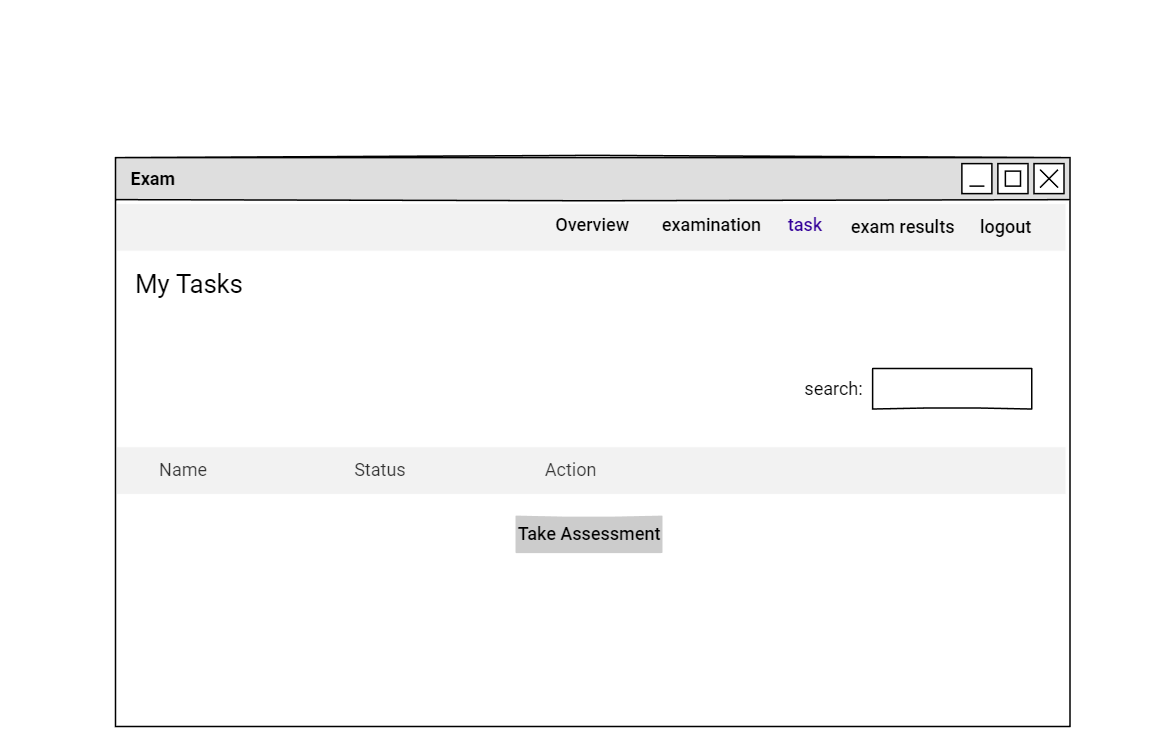
\includegraphics[width=.6\linewidth ]{img/user/userviewtask}
\caption{User View Tasks}
\end{figure}
\pagebreak
\subsection {User Submit Task}
Attend Tasks
\begin{figure}[bph]
	\centering
	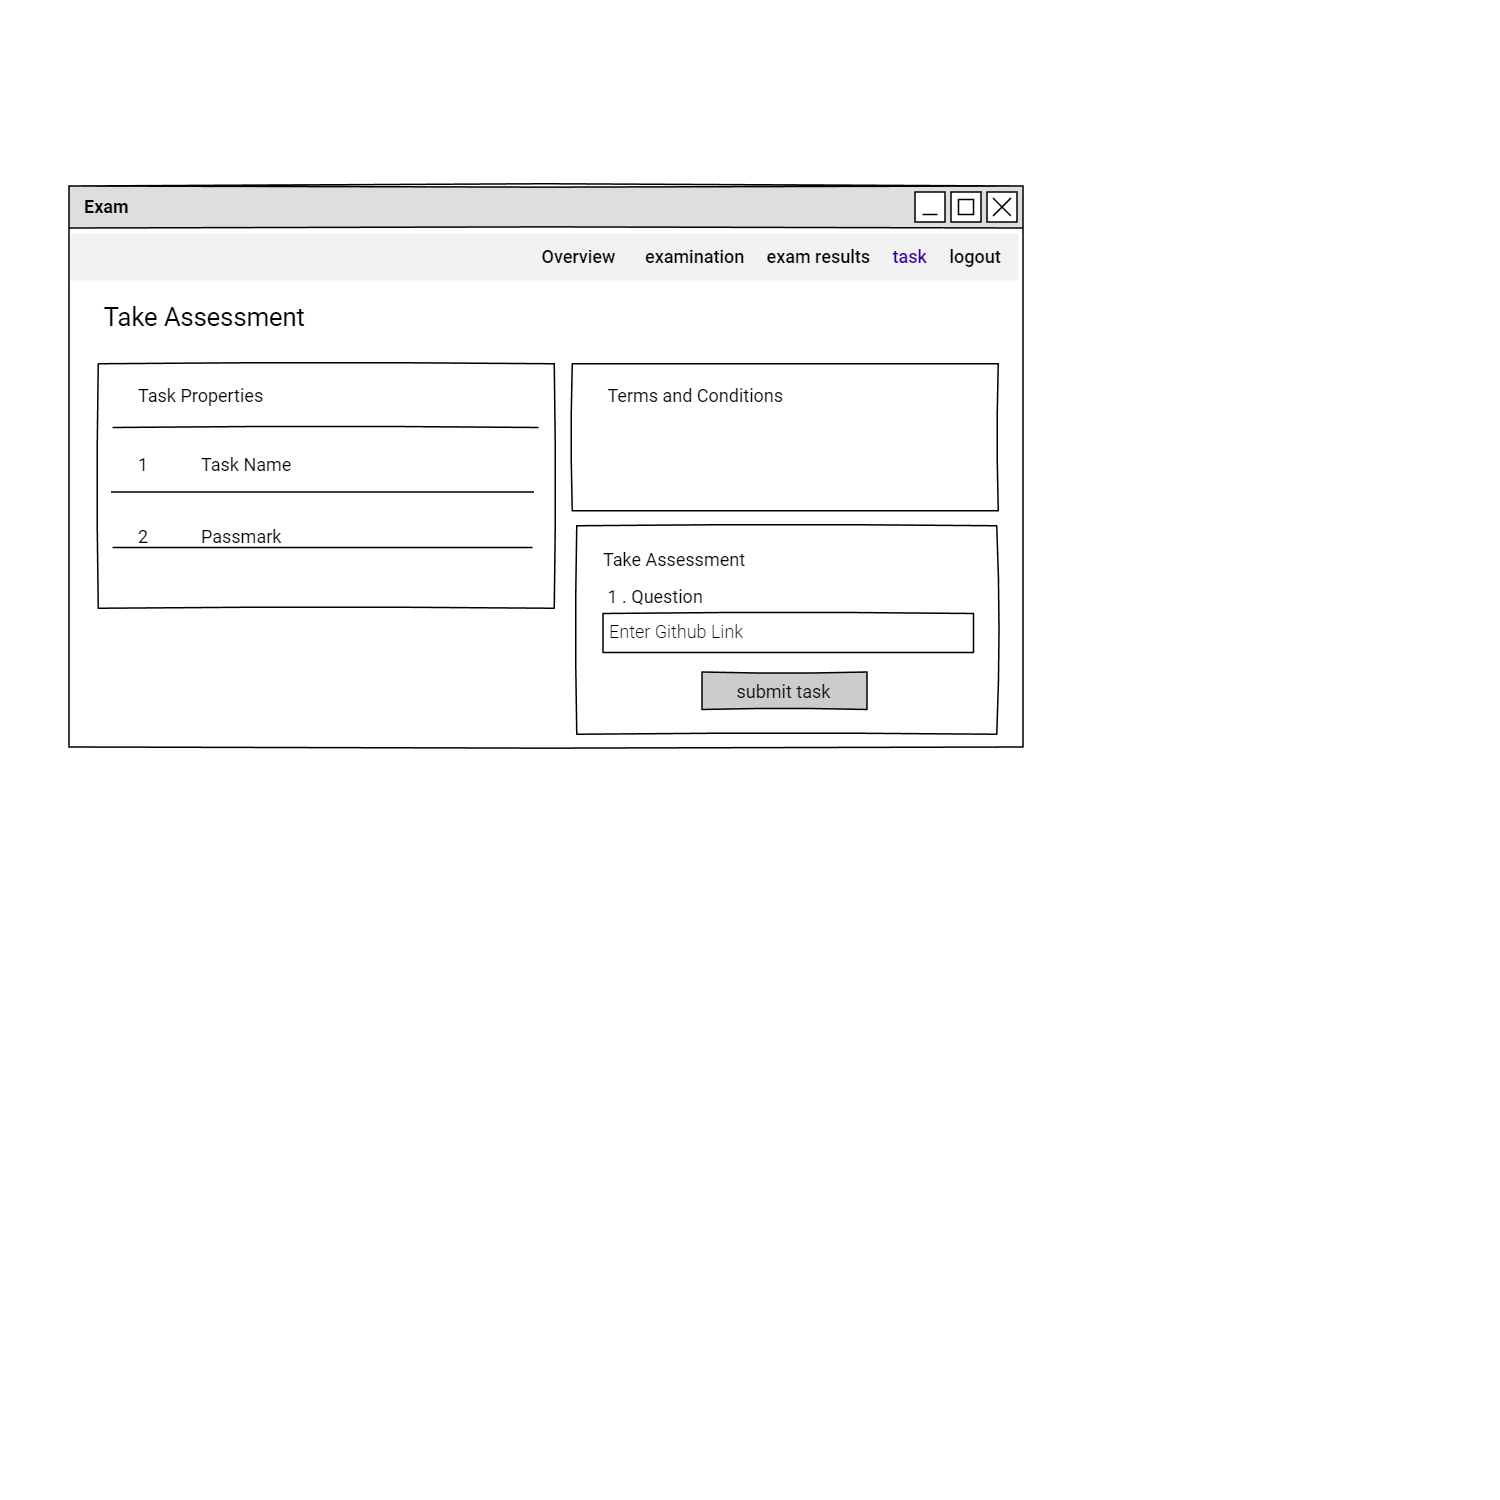
\includegraphics[width=.6\linewidth ]{img/user/takeassessment}
	\caption{User Submit Task}
\end{figure}
\pagebreak
\subsection {User View Exam Results}
View Scores for Task and Exams
\begin{figure}[bph]
	\centering
	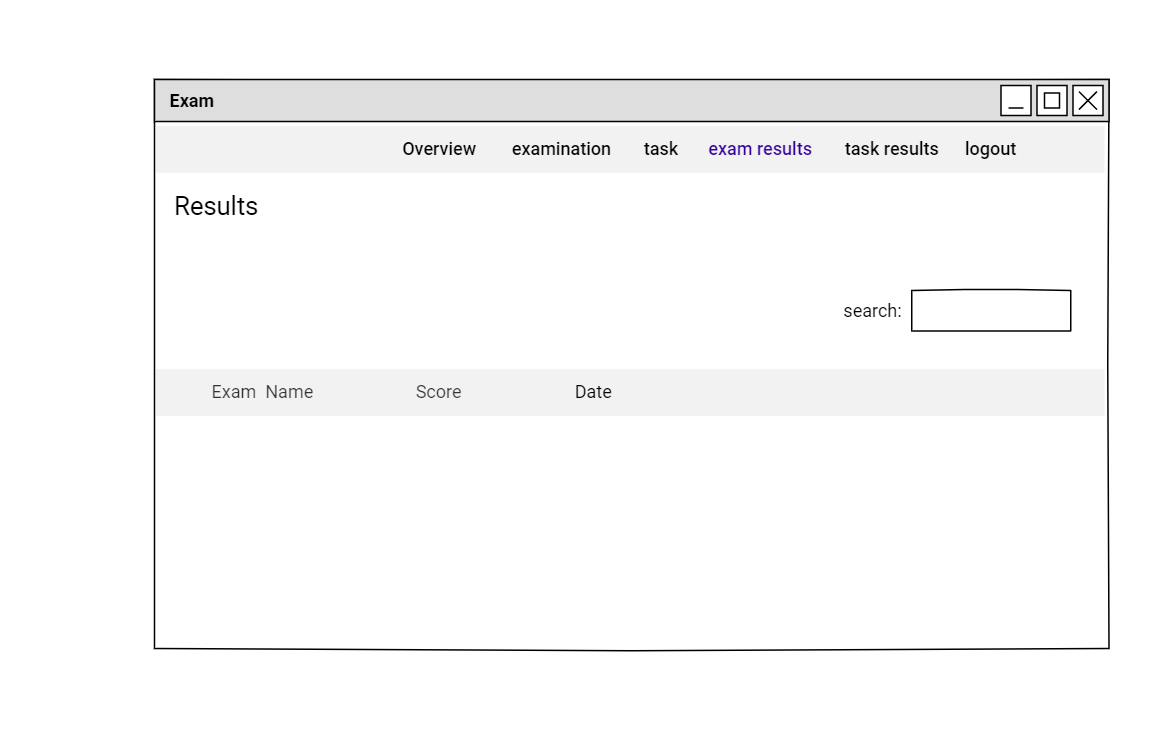
\includegraphics[width=.6\linewidth ]{img/user/usrexmrslt}
\caption{User View Exam Results}
\end{figure}
\subsection {User View Task Results}
View Scores for Task and Exams
\begin{figure}[bph]
	\centering
	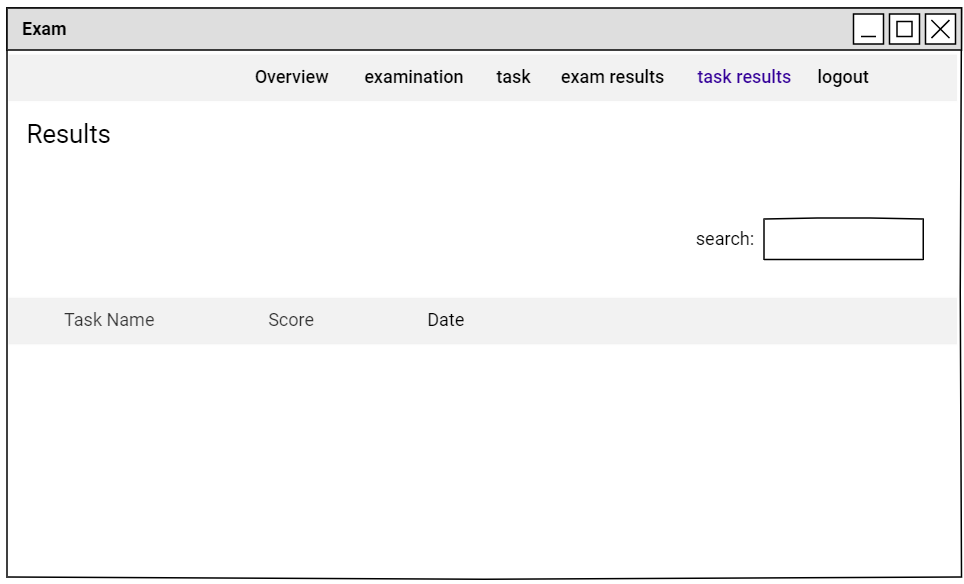
\includegraphics[width=.6\linewidth ]{img/user/usrtskrslt}
	\caption{User View Task Results}
\end{figure}
\pagebreak

\pagebreak
\subsection {Settings}
registered user can Change  Password   and also Delete Account if needed.
\begin{figure}[bph]
	\centering
	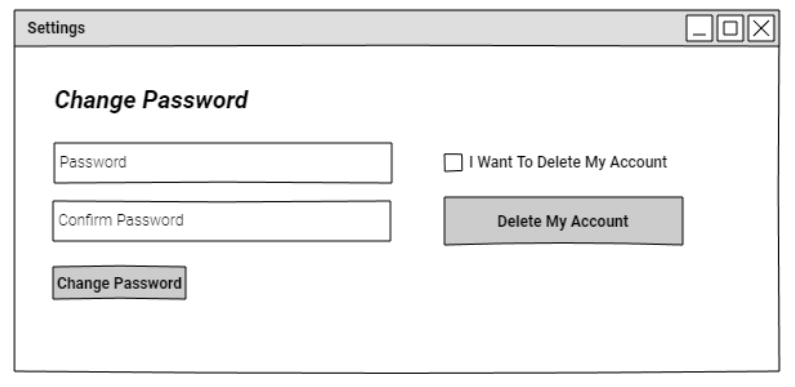
\includegraphics[width=.6\linewidth ]{img/user/changeuserpassword}
	\caption{Settings}
\end{figure}

\addcontentsline{toc}{section}{ - Company}
\subsection {Company Registration}
Registration form for company
\begin{figure}[bph]
	\centering
	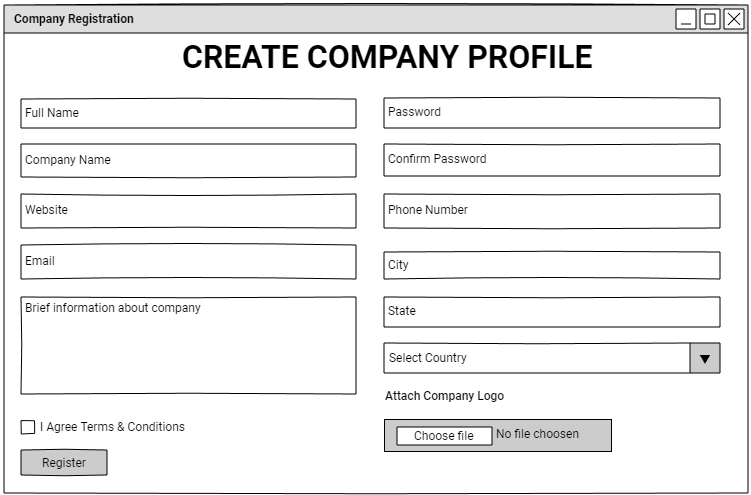
\includegraphics[width=.8\linewidth ]{img/company/company_registration}
	\caption{Company Registration}
\end{figure}
\pagebreak
\subsection {Dashboard}
Dashboard for company
\begin{figure}[bph]
	\centering
	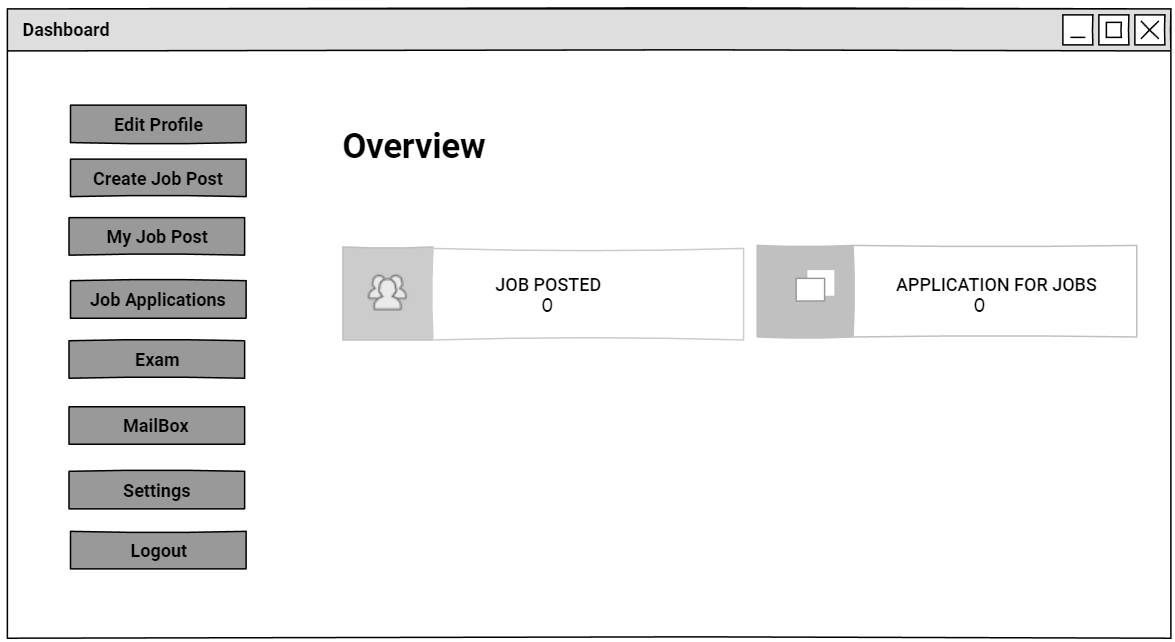
\includegraphics[width=1\linewidth]{img/company/untitled_page}
	\caption{Dashboard}
\end{figure}

\pagebreak
\subsection {Edit Profile}
Edit Company details
\begin{figure}[bph]
	\centering
	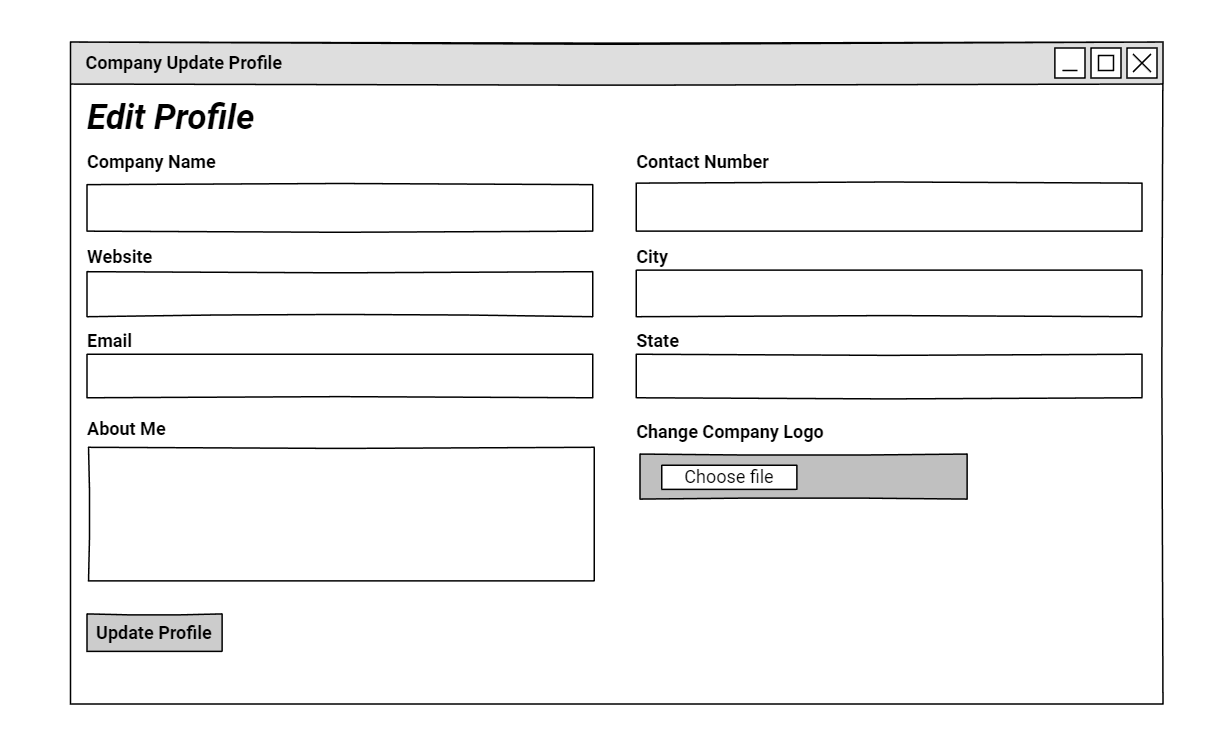
\includegraphics[width=.6\linewidth]{img/company/cmpnyprflupdt}
		\caption{Edit Profile}
\end{figure}

\subsection {Create Job Post}
Create New Job Posts with Details
\begin{figure}[bph]
	\centering
	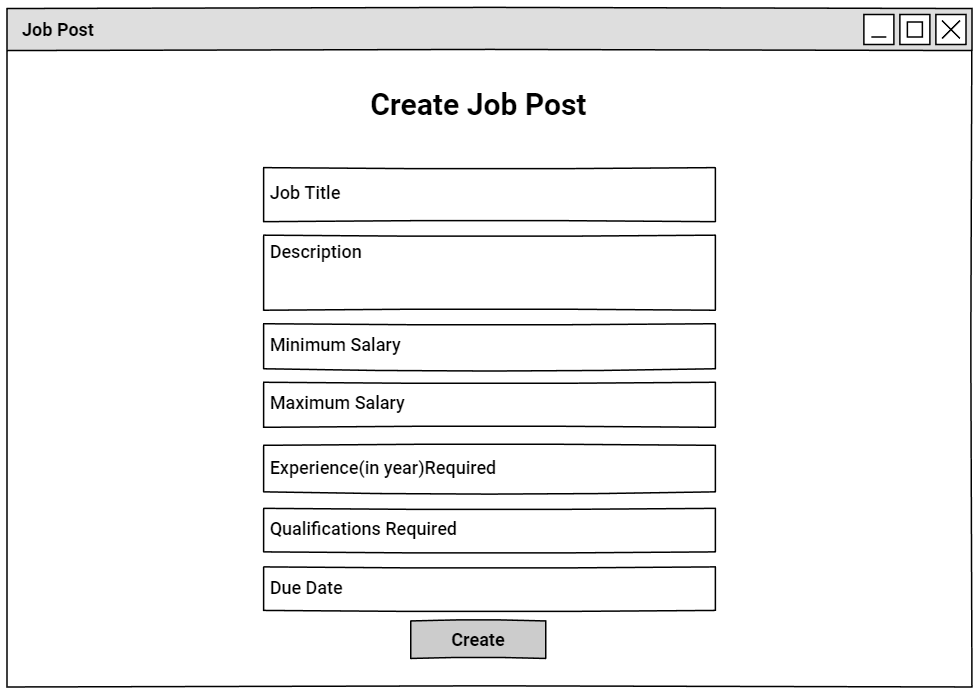
\includegraphics[width=.6\linewidth]{img/company/postjob}
	\caption{Create Job Post}
\end{figure}
\pagebreak
\subsection {Job Posts}
View posted Jobs by Company
\begin{figure}[bph]
	\centering
	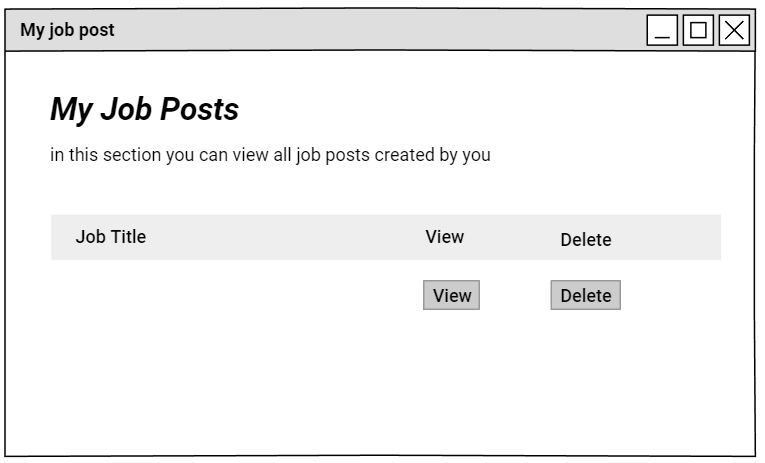
\includegraphics[width=.6\linewidth]{img/company/postedjobs}
	\caption{Job Posts}
\end{figure}

\subsection {Job Applications}
View Job Post Applications from Users and Review
\begin{figure}[bph]
	\centering
	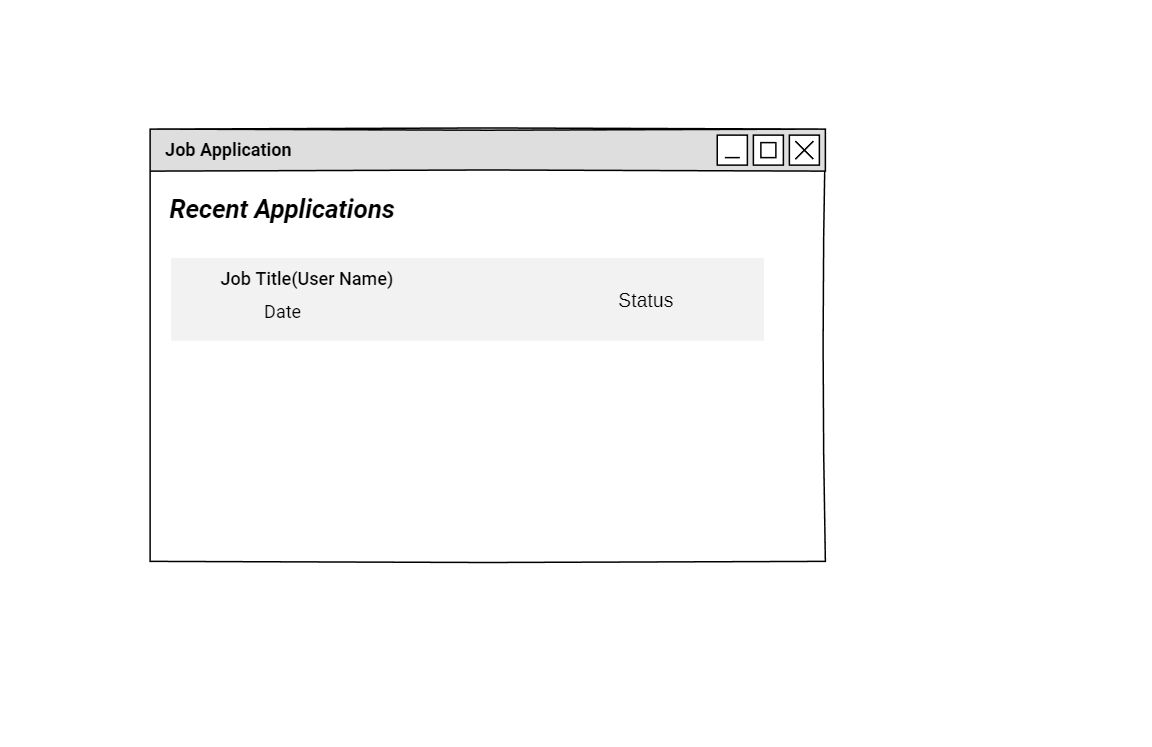
\includegraphics[width=.7\linewidth]{img/company/jobapltns}
	\caption{Job Applications}
\end{figure}
\pagebreak

\subsection {Download Resumes}
Download Resumes of Applied Users for Company's Job Posts
\begin{figure}[bph]
	\centering
	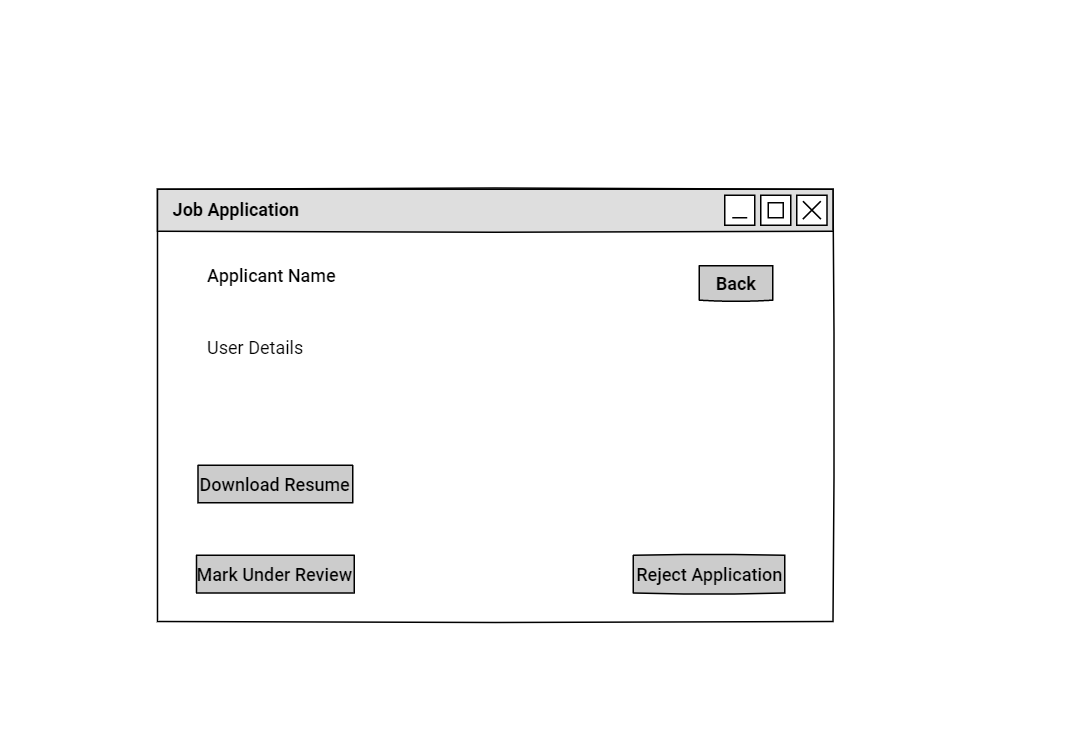
\includegraphics[width=.7\linewidth]{img/company/download_resume}
	\caption{Download Resume}
\end{figure}
\pagebreak
\subsection {Company View all Exam }
Using this form company can view all eaxams and search any candidate's exam score who attend the task.
\begin{figure}[bph]
	\centering
	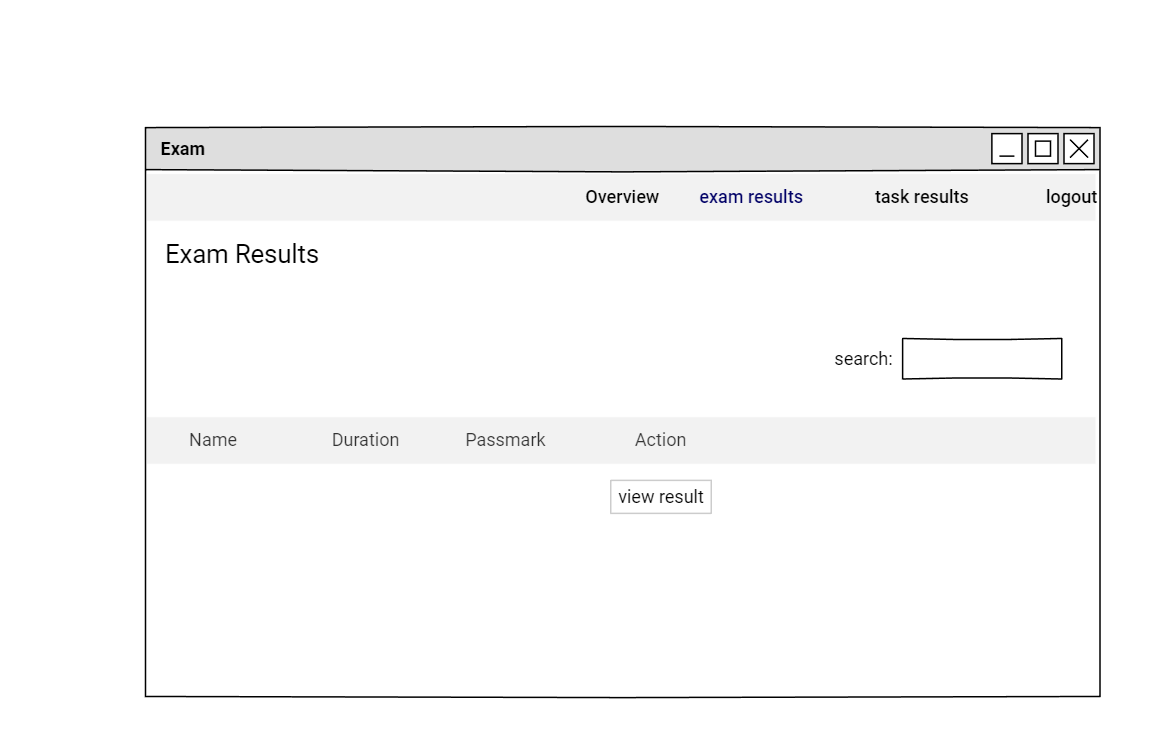
\includegraphics[width=.6\linewidth]{img/company/ce1}
	\caption{Company View all Exam}
\end{figure}
\pagebreak
\subsection {Company View Exam  Score}
Using this form company can view any candidate's exam score who attend the exam.
\begin{figure}[bph]
	\centering
	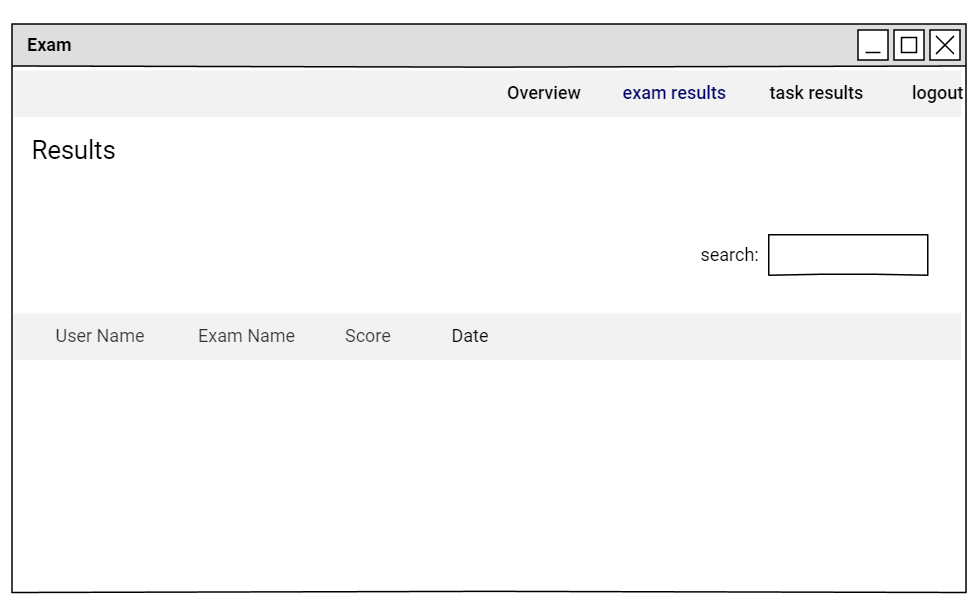
\includegraphics[width=.6\linewidth]{img/company/cmpnyviewsinlexmrslt}
	\caption{Company  Exam  Score}
\end{figure}
\pagebreak
\subsection {Company View All Task }
Using this form company can view all tasks and search any candidate's task score who submit the task.
\begin{figure}[bph]
	\centering
	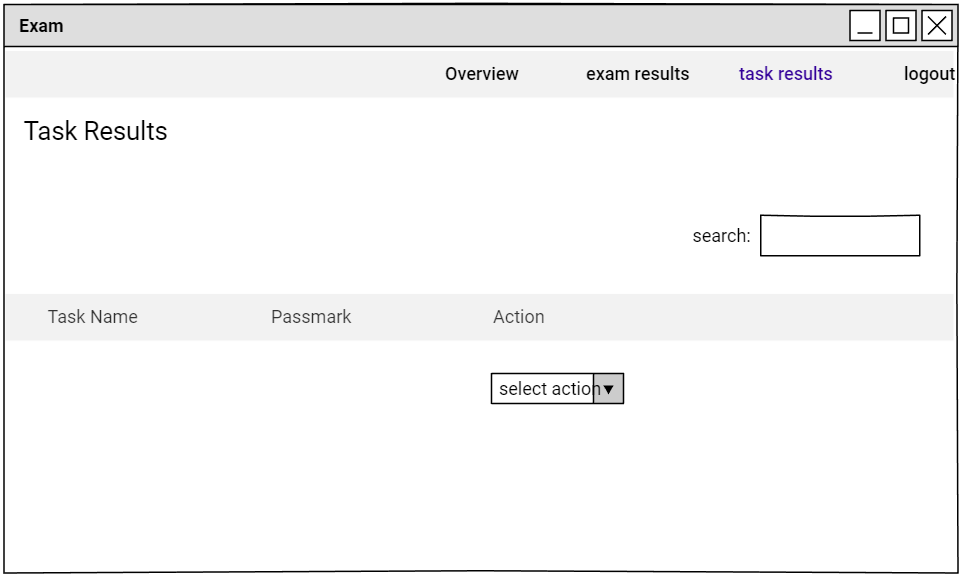
\includegraphics[width=.7\linewidth]{img/company/ct1}
	\caption{Company View All Task }
\end{figure}
\pagebreak
\subsection {Company View Task Scores }
Using this form company can view any candidate's task score who submit the task.
\begin{figure}[bph]
	\centering
	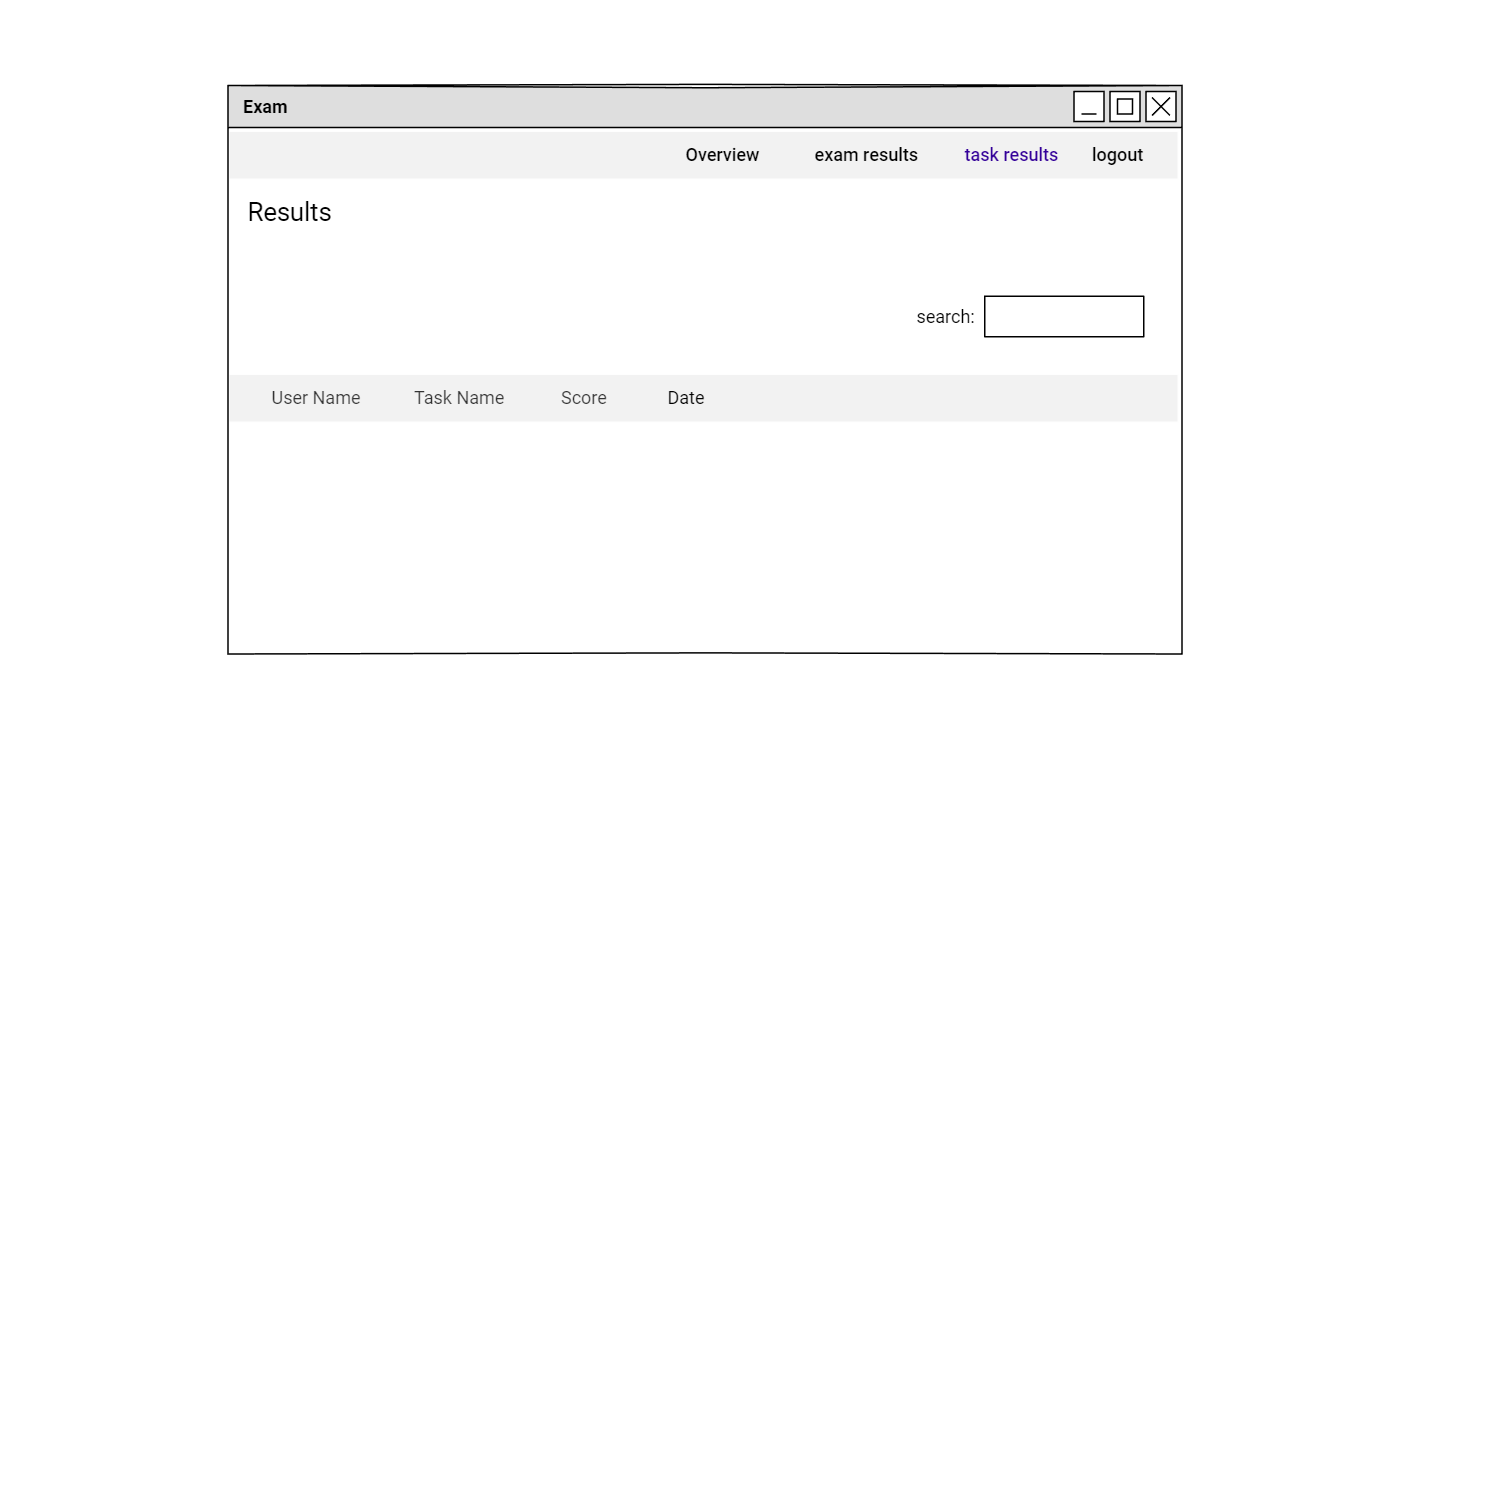
\includegraphics[width=.7\linewidth]{img/company/ct2}
	\caption{Company View Task Scores }
\end{figure}
\pagebreak
\subsection {Settings}
 registered company can Change FullName or Password of Company and also Delete Account if needed.
\begin{figure}[bph]
	\centering
	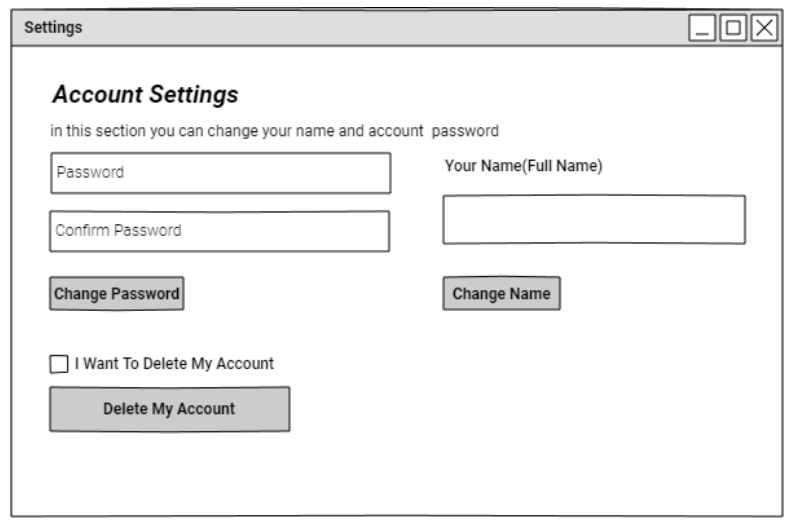
\includegraphics[width=.6\linewidth]{img/company/changecmpnypassword}
	\caption{Settings}
\end{figure}
\pagebreak
\addcontentsline{toc}{section}{ - Admin}
\subsection {Admin Homepage}
Overview of WorkLord with Registered Companies, User, Job Post, etc.. 
\begin{figure}[bph]
	\centering
	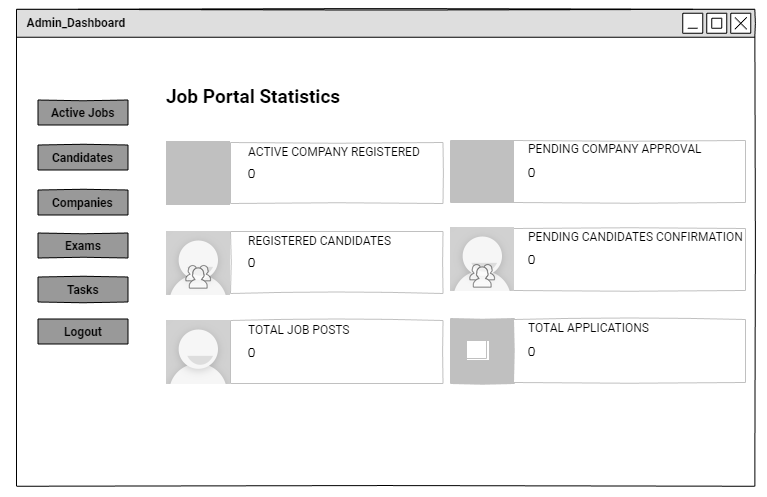
\includegraphics[width=1\linewidth]{img/admin/admindash}
	\caption{Admin Homepage}
\end{figure}


\pagebreak

\subsection {Active Jobs}
Admin can active or reject job vaccancies posted by different companies. 
\begin{figure}[bph]
	\centering
	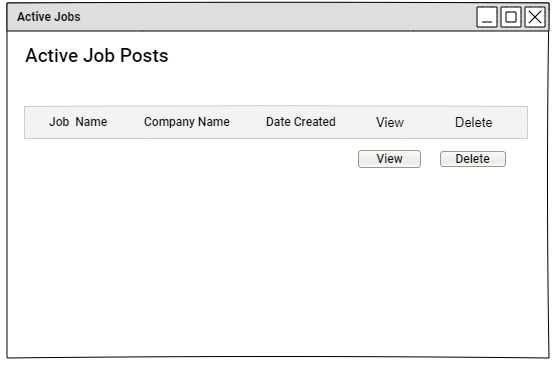
\includegraphics[width=.6\linewidth]{img/admin/adminavtvejobs}
	\caption{Active Jobs}
\end{figure}

\subsection {Candidates}
Show candidates details that are registered in the website and also can download the resume of each cadidates.
\begin{figure}[bph]
	\centering
	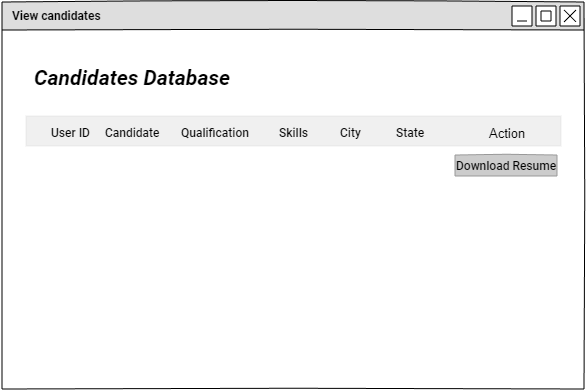
\includegraphics[width=.6\linewidth]{img/admin/adminviewcandidts}
	\caption{Candidates}
\end{figure}
\pagebreak

\subsection {Companies}
Show company details that are registered in the website and also can approve or rejact the registration of each company.
\begin{figure}[bph]
	\centering
	\includegraphics[width=.8\linewidth]{img/admin/adminviewcmpny}
	\caption{Companies}
\end{figure}
\pagebreak
\subsection {Admin Exam Dashboard}
Show details of exams.
\begin{figure}[bph]
	\centering
	\includegraphics[width=.6\linewidth]{img/admin/overview}
	\caption{Admin Exam Dashboard}
\end{figure}
\pagebreak

\subsection {Admin View  Exams}
View alla exams created by admin.
\begin{figure}[bph]
	\centering
	\includegraphics[width=.5\linewidth]{img/admin/e1}
	\caption{Admin View  Exams}
\end{figure}
\subsection {Admin Add Exams}
Admin can create new exam with exam name,duration, terms and conditions and passmark.
\begin{figure}[bph]
	\centering
	\includegraphics[width=.5\linewidth]{img/admin/add_exam}
	\caption{Admin Add Exams}
\end{figure}
\pagebreak
\subsection {Add Questions}
Add Questions for Exams
\begin{figure}[bph]
	\centering
	\includegraphics[width=.5\linewidth]{img/admin/addexmqstn}
	\caption{Add Questions}
\end{figure}
\pagebreak
\subsection {View Exam  Questions}
Using this form admin can view questions of each exams and also can upadate and delete questions.
\begin{figure}[bph]
	\centering
	\includegraphics[width=.5\linewidth]{img/admin/viweexmqstn}
	\caption{View Exam  Questions}
\end{figure}


\pagebreak
\subsection { View Tasks}
View alla task created by admin.
\begin{figure}[bph]
	\centering
	\includegraphics[width=.55\linewidth]{img/admin/t1}
	\caption{ View Tasks}
\end{figure}
\pagebreak

\subsection {Add Tasks}
 Admin can create new tasks with task name,question, terms and conditions and passmark.
\begin{figure}[bph]
	\centering
	\includegraphics[width=.6\linewidth]{img/admin/addtask}
	\caption{Add Tasks}
\end{figure}
\pagebreak
\subsection {View Task Question}
Using this form admin can view question of each task.
\begin{figure}[bph]
	\centering
	\includegraphics[width=.6\linewidth]{img/admin/viewtaskqstn}
	\caption{View Task Question}
\end{figure}
\pagebreak
\subsection { Admin View All Exam Scores}
This form list all task created by admin.By selecting action admin can view candidate's  task score of each task. 
\begin{figure}[bph]
	\centering
	\includegraphics[width=.6\linewidth]{img/admin/adviewallxmrslt}
	\caption{ Admin View All Exam Scores}
\end{figure}
\pagebreak
\subsection { Admin View Particular Exam Scores}
Admin can view scores of particular task submited by candidates. 
\begin{figure}[bph]
	\centering
	\includegraphics[width=.6\linewidth]{img/admin/adminviewrsltofparticlrxam}
	\caption{Admin View Particular Exam Scores}
\end{figure}
\pagebreak
\subsection { Admin View All Task Scores}
This form list all task created by admin.By selecting action admin can view candidate's  task score of each task. 
\begin{figure}[bph]
	\centering
	\includegraphics[width=.6\linewidth]{img/admin/adviewalltskrslt}
	\caption{Admin View All Task Scores}
\end{figure}
\pagebreak
\subsection { Admin View Particular Task Scores}
Admin can view scores of particular task submited by candidates. 
\begin{figure}[bph]
	\centering
	\includegraphics[width=.6\linewidth]{img/admin/adview_singletskrslt}
	\caption{Admin View Particular Task Scores}
\end{figure}
\pagebreak
\subsection { View Tasks For  Review}
This form list all the tasks one by one created by admin.by selecting action admin can view list of candidates they submit particular task.
\begin{figure}[bph]
	\centering
	\includegraphics[width=.8\linewidth]{img/admin/rvwtask1}
	\caption{T View Tasks For  Review}
\end{figure}

\pagebreak
\subsection {   Review  Tasks}
This form list all candidate they submit a particular task.from which admin can move to reviewing each task.
\begin{figure}[bph]
	\centering
	\includegraphics[width=.8\linewidth]{img/admin/rvwtsk2}
	\caption{Review  Tasks}
\end{figure}

\pagebreak
\subsection {  Enter Task Score}
Admin can evaluate the task submited by candidates by evaluating the githublink and upload the score for their task using this form.This form also display task question and it's properties.
\begin{figure}[bph]
	\centering
	\includegraphics[width=.8\linewidth]{img/admin/rvwtsk3}
	\caption{Enter Task Score}
\end{figure}

\pagebreak

\chapter{TESTING AND IMPLEMENTATION}

\section{Testing}
\subsection{Test Case - 1 }

\begin{center}
	\begin{tabular}{ | p {.5 cm} | p {2 cm} | p {2 cm} |  p {3 cm} |  p {3 cm} |  p {1 cm} |}		
		\hline
		\centering	\bf No. &
		\bf Date  &
		\bf Action &
		\bf Expected Result& 
		\bf Actual Result &
		\bf Pass? \\
		\hline

		1&15-09-2020& Home page  & Admin/ Company/
		 Candidates can view the type of services.
		  & Admin/ Company/ Candidates can view the type of services. & Yes  \\ \hline
		2&18-09-2020 & Registration  & Company/ Candidates should be able to register into the System  & Company/ Candidates should be able to register into the System &  Yes  \\ \hline
		3&20-09-2020& Login & Users of the system can able to login to the system  & Users of the system can able to login to the system &  Yes  \\ \hline
		4& 23-09-2020 & View companies & Admin can view the companies register in the system & Admin can view the companies register in the system &  Yes  \\ \hline
		5& 27-09-2020 & Approve/ Disapprove Company & Admin can approve or reject or reactivate company registration  & Admin can approve or reject or reactivate  company registration &  Yes  \\ \hline


	\end{tabular}
	\captionof{table}{ Test Case - 1}
\end{center}
\pagebreak

\subsection{Test Case - 2 }

\begin{center}
	\begin{tabular}{ | p {.5 cm} | p {2 cm} | p {2 cm} |  p {3 cm} |  p {3 cm} |  p {1 cm} |}		
		\hline
		\centering	\bf No. &
		\bf Date  &
		\bf Action &
		\bf Expected Result& 
		\bf Actual Result &
		\bf Pass? \\
		\hline

		6&30-09-2020& Post Jobs  & Employer can post job vacancies in their company
		& Employer can post job vacancies in their company. & Yes  \\ \hline

		7&04-10-2020 & View and Delete Jobs  & Admin can view and delete job post & Admin can view and delete job post &  Yes  \\ \hline

		8&10-10-2020& Search, view, apply jobs and view applied job applications & Users can view, search and apply for jobs and also view their applied job applications & Users can view, search and apply for jobs and also view their applied job applications &  Yes  \\ \hline

		9& 11-10-2020 & View Posted Jobs & Companies can view and delete their posted job vacancies &Companies can view and delete their posted job vacancies &  Yes  \\ \hline


	\end{tabular}
	\captionof{table}{ Test Case - 2}
\end{center}
\pagebreak

\subsection{Test Case - 3 }

\begin{center}
	\begin{tabular}{ | p {.5 cm} | p {2 cm} | p {2 cm} |  p {3 cm} |  p {3 cm} |  p {1 cm} |}		
		\hline
		\centering	\bf No. &
		\bf Date  &
		\bf Action &
		\bf Expected Result& 
		\bf Actual Result &
		\bf Pass? \\
		\hline

		10&14-10-2020&View Job Applications And Download resumes  & Employer can view job application for their job post applied by different candidates and also employer can download their resumes.
		& Employer can view job application for their job post applied by different candidates and also employer can download their resumes. & Yes  \\ \hline

		11&19-10-2020 & Create Exams  & Admin can create exam, add questions and also manage created exams.  & Admin can create exam, add questions and also manage created exams &  Yes  \\ \hline

		12&22-10-2020& Create Tasks & Admin can create Tasks, add questions and also manage created tasks & Admin can create Tasks, add questions and also manage created tasks. &  Yes  \\ \hline

		13&30-10-2020 &	Attend Exam & User can attend exams. & User can attend exams. &  Yes  \\ \hline


	\end{tabular}
	\captionof{table}{ Test Case - 3}
\end{center}
\pagebreak

\subsection{Test Case - 4 }

\begin{center}
	\begin{tabular}{ | p {.5 cm} | p {2 cm} | p {2 cm} |  p {3 cm} |  p {3 cm} |  p {1 cm} |}		
		\hline
		\centering	\bf No. &
		\bf Date  &
		\bf Action &
		\bf Expected Result& 
		\bf Actual Result &
		\bf Pass? \\
		\hline

		14&31-10-2020&View candidates & Admin can view registered candidates details.& Admin can view registered candidates details. & Yes  \\ \hline

		15&04-11-2020 & Attend Task & User can submit task & User can submit task &  Yes  \\ \hline

		16&11-11-2020& View Exam, Task Scores, Review tasks & Admin/ user/ company can view candidate’s exam and task scores. & Admin/ user/ company can view candidate’s exam and task scores. &  Yes  \\ \hline

		17&13-11-2020 &	Send/ Receive Messages & user/ company can send or receive messages. & user/ company can send or receive messages. &  Yes  \\ \hline

		18&15-11-2020 &	Update profile and change password & User/ company can update their profile and can change password. & User/ company can update their profile and can change password. &  Yes  \\ \hline


	\end{tabular}
	\captionof{table}{ Test Case - 4}
\end{center}
\pagebreak
\section{Implementation}

After testing, the proposed system is ready for the implementation. Implementation is the stage of the project when the theoretical design is turned in to a working
system. Implementation is the process of bringing a newly developed system or revised into operational one. The new system and its components are to be tested in a structured and planned manner. The implementation stage of a project is often very
complex and time consuming and many more people are involved in the earlier stages.
This involves careful planning, investigation of the current system and constraints of implementation, installing hardware, training the operating users in the changeover procedures before the system is setup and running. So, proposed system is easy to implement. It would be very easy to run also.\\

While implementing this system we only have few challenges. First challenge is to provide access to this webpage from anywhere or any device with internet access. For that we had to host the webpage in server with database access. If number users increase in this situation it won't affect as much as hosting in a local server. Most Hosting Providers have highly capable bandwidth and powerful computer to handle such traffic. The user must have a device with brower and stable internet access. Rest of the challenges are depended on the user, knowledge about using an electronic device and using it for accessing website. \\

\pagebreak

\chapter{CONCLUSION}

\pagebreak

\chapter{REFERENCES}

\begin{enumerate}
\item - M. Mansourvar and N. Y. Mohd, “Web portal as a knowledge management system in the universities,” World Academy of Science,Engineering and Technology, 2010.
\item - S. Mauno, U. Kinnunen, and M. Ruokolainen, “Job demands and resources as antecedents of work engagement: A longitudinal study,” Journal of Vocational Behavior, 2007.
\item - A. Doyle, Internet Your Way to a New Job: How to Really Find a Job Online, Happy about, 2008.
\item - N. Sulaiman and M. Burke, “A case analysis of knowledge sharing implementation and job searching in Malaysia,” International Journal of Information Management, 2009.
\item - M. Mansourvar, Development of a Job Web Portal to Capture Industry’s Needs, 2011.
\item - M. Mansourvar and N. B. M. Yasin, “Knowledge portal: a tool to capture university requirements,” in Proc. 2011 International Conf. on Graphic and Image Processing, International Society for Optics and Photonics, October 2011.

	\item - https://stackoverflow.com
	\item - https://www.w3schools.com
	\item - https://www.tutorialspoint.com/php/index.htm
	\item - https://getbootstrap.com
	\item - https://jqueryvalidation.org/documentation/
	\item - https://www.php.net/manual/en/book.mysqli.php
	\item - https://www.apachefriends.org/index.html
	\item -	https://mariadb.com/kb/en/documentation/
	\item -	https://www.000webhost.com/forum/
	\item -	https://docs.github.com/en
	\item -	https://git-scm.com/doc
\end{enumerate} 
\pagebreak

\chapter{APPENDIX}


\section{Source Code}

\subsection{Country, State and City Selection in Registration}
\begin{verbatim}

<div class="form-group">
<select class="form-control  input-lg" id="country" name="country" 
required>
<option selected="" value="">Select Country</option>
<?php
$sql="SELECT * FROM countries";
$result=$conn->query($sql);

if($result->num_rows > 0) {
	while($row = $result->fetch_assoc()) {
		echo "<option value='".$row['name']."' 
        data-id='".$row['id']."'>".$row['name']."</option>";
	}
}
?>

</select>
</div>  
<div id="stateDiv" class="form-group" style="display: none;">
<select class="form-control  input-lg" id="state" name="state" 
required>
<option value="" selected="">Select State</option>
</select>
</div>   
<div id="cityDiv" class="form-group" style="display: none;">
<select class="form-control  input-lg" id="city" name="city" >
<option selected="">Select City</option>
</select>
</div>

<script>
$("#country").on("change", function() {
	var id = $(this).find(':selected').attr("data-id");
	$("#state").find('option:not(:first)').remove();
	if(id != '') {
		$.post("state.php", {id: id}).done(function(data) {
			$("#state").append(data);
		});
		$('#stateDiv').show();
	} else {
		$('#stateDiv').hide();
		$('#cityDiv').hide();
	}
});
</script>

<script>
$("#state").on("change", function() {
	var id = $(this).find(':selected').attr("data-id");
	$("#city").find('option:not(:first)').remove();
	if(id != '') {
		$.post("city.php", {id: id}).done(function(data) {
			$("#city").append(data);
		});
		$('#cityDiv').show();
	} else {
		$('#cityDiv').hide();
	}
});
</script>

$sql = "SELECT * FROM states WHERE country_id='$_POST[id]'";
$result = $conn->query($sql);

if($result->num_rows > 0) {
	while($row = $result->fetch_assoc()) {		
		echo '<option value="'.$row["name"].'"
        data-id="'.$row["id"].'">'.$row["name"].'</option>';		
	}	
}

$sql = "SELECT * FROM cities WHERE state_id='$_POST[id]'";
$result = $conn->query($sql);
if($result->num_rows > 0) {
	while($row = $result->fetch_assoc()) {	
		echo '<option value="'.$row["name"].'"
	    data-id="'.$row["id"].'">'.$row["name"].'</option>';	
	}	
}

\end{verbatim}

\subsection{Showing Random Job Posts in Homepage}

\begin{verbatim}
<section id="jobs" class="jobs">
<div class="container" data-aos="fade-up">

<div class="section-title">
<h2>Jobs</h2>
<div class="row">
<div class="col-md-12 text-center index-head">
<h1>“If you can <strong>DREAM</strong> it, you can DO it ”</h1>
<p><a class="btn btn-success btn-lg" href="jobs.php"
 role="button">Search Jobs</a></p>
</div>
</div>
</div>
<div class="row">
<div class="col-md-12 latest-job margin-bottom-20">
<?php 
$today = (new DateTime())->format('Y-m-d');
$sql = "SELECT * FROM job_post WHERE duedate<='$today'
and active=1 Order By Rand() Limit 4";
$result = $conn->query($sql);
if($result->num_rows > 0) {
	while($row = $result->fetch_assoc()) 
	{
		$sql1 = "SELECT * FROM company WHERE id_company='$row[id_company]'";
		$result1 = $conn->query($sql1);
		if($result1->num_rows > 0) {
			while($row1 = $result1->fetch_assoc()) 
			{
				?>
				<div class="clearfix">
				<div>
				<h4><a href="view-job-post.php?id=<?php echo $row['id_jobpost'];
				?>"><?php echo $row['jobtitle']; ?></a> <span class="pull-right">
				<?php echo $row['maximumsalary']; ?>/Month</span></h4>
				<div>
				<div><strong><?php echo $row1['companyname']; ?> | 
				<?php echo $row1['city']; ?> | 
				Experience <?php echo $row['experience']; ?> 
				Years</strong></div>
				</div></div></div>
				<?php
			}}}}
?>
</div></div></div></section>

\end{verbatim}

\subsection{User Registration}

\begin{verbatim}
<?php
//To Handle Session Variables on This Page
session_start();
//Including Database Connection From db.php
require_once("db.php");
//If user Actually clicked register button
if(isset($_POST)) {
	//Escape Special Characters In String First
	$firstname = mysqli_real_escape_string($conn, $_POST['fname']);
	$lastname = mysqli_real_escape_string($conn, $_POST['lname']);
	$address = mysqli_real_escape_string($conn, $_POST['address']);
	$city = mysqli_real_escape_string($conn, $_POST['city']);
	$state = mysqli_real_escape_string($conn, $_POST['state']);
	$contactno = mysqli_real_escape_string($conn, $_POST['contactno']);
	$qualification=
	mysqli_real_escape_string($conn,$_POST['qualification']);
	$stream = mysqli_real_escape_string($conn, $_POST['stream']);
	$passingyear=mysqli_real_escape_string($conn, $_POST['passingyear']);
	$dob = mysqli_real_escape_string($conn, $_POST['dob']);
	$age = mysqli_real_escape_string($conn, $_POST['age']);
	$designation=mysqli_real_escape_string($conn, $_POST['designation']);
	$aboutme = mysqli_real_escape_string($conn, $_POST['aboutme']);
	$skills = mysqli_real_escape_string($conn, $_POST['skills']);
	$email = mysqli_real_escape_string($conn, $_POST['email']);
	$password = mysqli_real_escape_string($conn, $_POST['password']);
	//Encrypt Password
	$password = base64_encode(strrev(md5($password)));
	//sql query to check if email already exists or not
	$sql = "SELECT email FROM users WHERE email='$email'";
	$result = $conn->query($sql);
	
	//if email not found then we can insert new data
	if($result->num_rows == 0) {
		//This variable is used to catch errors doing upload process.
		$uploadOk = true;
		//Folder where you want to save your resume.
		$folder_dir = "uploads/resume/";
		//Getting Basename of file.
		$base = basename($_FILES['resume']['name']); 
		//This will get us extension of your file.
		$resumeFileType = pathinfo($base, PATHINFO_EXTENSION); 
		//Setting a random non repeatable file name. 
		$file = uniqid() . "." . $resumeFileType;   
		//This is where your files will be saved
		$filename = $folder_dir .$file;  
		//We check if file is saved to our temp location or not.
		if(file_exists($_FILES['resume']['tmp_name'])) { 
			//checks if file type is allowed or not.
			if($resumeFileType == "pdf")  {
				//check file size with our limit size.
				if($_FILES['resume']['size'] < 500000) {
					//If condition are met then copy file
					move_uploaded_file($_FILES["resume"]["tmp_name"], $filename);
				} else {
					//Size Error
					$_SESSION['uploadError'] = "Wrong Size. Max Size Allowed : 5MB";
					$uploadOk = false;
				}
			} else {
				//Format Error
				$_SESSION['uploadError'] = "Wrong Format. Only PDF Allowed";
				$uploadOk = false;
			}
		} else {
			//File not copied to temp location error.
			$_SESSION['uploadError'] = 
			"Something Went Wrong. File Not Uploaded. Try Again.";
			$uploadOk = false;
		}
		//If there is any error then redirect back.
		if($uploadOk == false) {
			header("Location: register-candidates.php");
			exit();
		}
		//sql new registration insert query
		$sql = "INSERT INTO users(firstname, lastname, email, address,
		city, state, contactno, qualification, stream, 
		passingyear, dob, age, designation, resume, aboutme, skills) 
		VALUES ('$firstname', '$lastname', '$email', '$address', '$city',
		'$state', '$contactno', '$qualification', '$stream',
		 '$passingyear','$dob', '$age', '$designation', '$file',
		  '$aboutme', '$skills')";
		$sql2 = "INSERT INTO login(email,password,role) 
		VALUES ('$email','$password','user')";
		if(($conn->query($sql))&&($conn->query($sql2))===TRUE) {	
			$_SESSION['uploadSuccess'] = "Registered Successfully";
			header("Location: login.php");
			exit();
		} else {
			//If data failed to insert then show that error.
			echo "Error " . $sql . "<br>" . $conn->error;
		}
	} else {
		//if email found in database then show email already exists error.
		$_SESSION['uploadError'] = "Already registered.";
		header("Location: register-candidates.php");
		exit();
	}
	//Close database connection. Not compulsory but good practice.
	$conn->close();
} else {
	header("Location: register-candidates.php");
	exit();
}
?>

\end{verbatim}

\subsection{Take Assessment}

\begin{verbatim}
<?php 
include '../../db.php';
$sql = "SELECT * FROM questions WHERE exam_id = '$exam_id'";
$result = $conn->query($sql);
if ($result->num_rows > 0) {
	while($row = $result->fetch_assoc()) {
		$qsid = $row['question_id'];
		$qs = $row['question'];
		$type = $row['type'];
		$op1 = $row['option1'];
		$op2 = $row['option2'];
		$op3 = $row['option3'];
		$op4 = $row['option4'];
		$ans = $row['answer'];
		$enan = $row[$ans];
		if ($type == "FB") {
			if ($qno == "1") {
				print '
				<div role="tabpanel" class="tab-pane active fade in"
				 id="tab'.$qno.'">
				<p><b>'.$qno.'.</b> '.$qs.'</p>
				<p><input type="text" name="an'.$qno.'"  class="form-control"
				 placeholder="Enter your answer" autocomplete="off">
				<input type="hidden" name="qst'.$qno.'"
				 value="'.base64_encode($qs).'">
				<input type="hidden" name="ran'.$qno.'"
				 value="'.base64_encode($ans).'">
				</div>
				';	
			}else{
				print '
				<div role="tabpanel" class="tab-pane fade in" id="tab'.$qno.'">
				<p><b>'.$qno.'.</b> '.$qs.'</p>
				<p><input type="text" name="an'.$qno.'"  class="form-control"
				 placeholder="Enter your answer" autocomplete="off">
				<input type="hidden" name="qst'.$qno.'"
				 value="'.base64_encode($qs).'">
				<input type="hidden" name="ran'.$qno.'"
				 value="'.base64_encode($ans).'">
				</div>
				';		
			}	
			$qno = $qno + 1;	
		}else{	
			if ($qno == "1") {		
				print '
				<div role="tabpanel" class="tab-pane active fade in"
				 id="tab'.$qno.'">
				<p><b>'.$qno.'.</b> '.$qs.'</p>
				<p><label class="container"><input type="radio" name="an'.$qno.'"
				  class="form-control container" value="'.$op1.'">
				   '.$op1.'</p></label>
				<p><label class="container"><input type="radio" name="an'.$qno.'"
				  class="form-control container" value="'.$op2.'">
				   '.$op2.'</p></label>
				<p><label class="container"><input type="radio" name="an'.$qno.'"
				  class="form-control container" value="'.$op3.'">
				   '.$op3.'</p></label>
				<p><label class="container"><input type="radio" name="an'.$qno.'"
				  class="form-control container" value="'.$op4.'">
				   '.$op4.'</p></label>
				<input type="hidden" name="qst'.$qno.'"
				 value="'.base64_encode($qs).'">
				<input type="hidden" name="ran'.$qno.'"
				 value="'.base64_encode($enan).'">
				</div>
				';	
			}else{
				print '
				<div role="tabpanel" class="tab-pane fade in" id="tab'.$qno.'">
				<p><b>'.$qno.'.</b> '.$qs.'</p>
				<p><label class="container"><input type="radio"
				 name="an'.$qno.'"  class="form-control container"
				  value="'.$op1.'"> '.$op1.'</p></label>
				<p><label class="container"><input type="radio"
				 name="an'.$qno.'"  class="form-control container"
				  value="'.$op2.'"> '.$op2.'</p></label>
				<p><label class="container"><input type="radio"
				 name="an'.$qno.'"  class="form-control container"
				  value="'.$op3.'"> '.$op3.'</p></label>
				<p><label class="container"><input type="radio"
				 name="an'.$qno.'"  class="form-control container"
				  value="'.$op4.'"> '.$op4.'</p></label>
				<input type="hidden" name="qst'.$qno.'"
				 value="'.base64_encode($qs).'">
				<input type="hidden" name="ran'.$qno.'"
				 value="'.base64_encode($enan).'">
				</div>
				';		
			}	
			$qno = $qno + 1;		
		}	}}
?>

\end{verbatim}

\subsection{Job Search}

\begin{verbatim}
	
<?php
session_start();
require_once("db.php");
$limit = 4;
if(isset($_GET["page"])) {
	$page = $_GET['page'];
} else {
	$page = 1;
}
$start_from = ($page-1) * $limit;
if(isset($_GET['filter']) && $_GET['filter']=='searchBar') {
	$search = $_GET['search'];
	$sql = "SELECT * FROM job_post WHERE jobtitle 
	LIKE '%$search%' LIMIT $start_from, $limit";
} else if(isset($_GET['filter']) 
&& $_GET['filter']=='experience') {
	$sql = "SELECT * FROM job_post WHERE active='1' 
	&& experience>='$_GET[search]' LIMIT $start_from, $limit";	
}
$result = $conn->query($sql);
if($result->num_rows > 0) {
	while($row = $result->fetch_assoc()) {
		$sql1 = "SELECT * FROM company WHERE id_company='$row[id_company]'";
		$result1 = $conn->query($sql1);
		if($result1->num_rows > 0) {
			while($row1 = $result1->fetch_assoc()) 
			{
				?>
				<div class="attachment-block clearfix">
				<img class="attachment-img" src="uploads/logo/<?php 
				echo $row1['logo']; ?>" alt="Attachment Image">
				<div class="attachment-pushed">
				<h4 class="attachment-heading"><a href="view-job-post.php?id=<?php 
				echo $row['id_jobpost']; ?>"><?php echo $row['jobtitle']; ?></a> 
				<span class="attachment-heading pull-right">
				<?php echo $row['maximumsalary']; ?>/Month</span></h4>
				<div class="attachment-text">
				<div><strong><?php echo $row1['companyname']; ?> |
				 <?php echo $row1['city']; ?> | Experience <?php 
				 echo $row['experience']; ?> Years</strong></div>
				</div></div></div>
				<?php
				}	}	}}

\end{verbatim}
\pagebreak

\section{Screenshots}

\subsection {Homepage}
This is the main page user sees when accessing {\bf Worklord} Job Portal Website. There will options to Login, Signup, Job Search and About (Motive of this project)
\begin{figure}[bph]
	\centering
	\includegraphics[width=.7\linewidth ]{img/screenshots/homepage}
	\caption{Homepage}
\end{figure}

\subsection {Jobs}
This section shows random Jobs Posted by different companies. Which Users and Guests can check details and Apply. Also provides option to search jobs
\begin{figure}[bph]
	\centering
	\includegraphics[width=.7\linewidth ]{img/screenshots/jobs}
	\caption{Jobs}
\end{figure}

\pagebreak

\subsection {About}
This section show the motive of this project, Importance of this project in our current scenario
\begin{figure}[bph]
	\centering
	\includegraphics[width=.7\linewidth ]{img/screenshots/about}
	\caption{About}
\end{figure}

\subsection {Login}
This is the login page for User, Company and Admin. This page checks the user's type and redirect to appropriate pages
\begin{figure}[bph]
	\centering
	\includegraphics[width=.7\linewidth ]{img/screenshots/login}
	\caption{Login}
\end{figure}

\pagebreak

\subsection {Register - Company}
This is the Registration page for every companies who are searching for new employees. Companies can register here with their details like email, company name, logo, etc.
\begin{figure}[bph]
	\centering
	\includegraphics[width=.7\linewidth ]{img/screenshots/comp_reg}
	\caption{Register - Company}
\end{figure}

\subsection {Register - User}
This is the Registration page for every users who are seeking for jobs. Users can register here with their details like email, name, resume, etc.
\begin{figure}[bph]
	\centering
	\includegraphics[width=.7\linewidth ]{img/screenshots/user_reg}
	\caption{Register - User}
\end{figure}

\pagebreak

\subsection {Users List}
This the page which admin can view all registered users in the Job Portal. Admin can check their profile details and view resumes
\begin{figure}[bph]
	\centering
	\includegraphics[width=.7\linewidth ]{img/screenshots/admin/users_list}
	\caption{Users List}
\end{figure}

\subsection {Company Management}
This the page which admin can view all registered companies in the Job Portal. Admin can check their profile details and Approve or Disapprove or Delete their registration request.
\begin{figure}[bph]
	\centering
	\includegraphics[width=.7\linewidth ]{img/screenshots/admin/company_mng}
	\caption{Company Management}
\end{figure}

\pagebreak

\subsection {Examinations}
This is the list of examinations, which admin is added for assessment of the users. Admin can View or Edit exam, Add or Remove questions and Drop exams.
\begin{figure}[bph]
	\centering
	\includegraphics[width=.7\linewidth ]{img/screenshots/admin/examslist}
	\caption{Examinations}
\end{figure}

\subsection {Add Exam}
In this page Admin can add exams for the users. Including duration of the exam and passmark for this exam.
\begin{figure}[bph]
	\centering
	\includegraphics[width=.7\linewidth ]{img/screenshots/admin/addexams}
	\caption{Add Exam}
\end{figure}

\pagebreak

\subsection {Tasks}
This is the list of Tasks, which admin is added for assessment of the users. Admin can view or edit tasks, view or change question and add drop tasks.
\begin{figure}[bph]
	\centering
	\includegraphics[width=.7\linewidth ]{img/screenshots/admin/tasks_list}
	\caption{Tasks}
\end{figure}

\subsection {Add Tasks}
In this page Admin can add Tasks for the users. Including question of the exam and passmark for this exam.
\begin{figure}[bph]
	\centering
	\includegraphics[width=.7\linewidth ]{img/screenshots/admin/addtasks}
	\caption{Add Tasks}
\end{figure}

\pagebreak


\subsection {Tasks Reviews List}
This is the list of Tasks to reviewed by the admin
\begin{figure}[bph]
	\centering
	\includegraphics[width=.7\linewidth ]{img/screenshots/admin/task_review2}
	\caption{Tasks Review}
\end{figure}

\subsection {Review Task}
In this page Admin can assign scores for the work users submitted through github.
\begin{figure}[bph]
	\centering
	\includegraphics[width=.7\linewidth ]{img/screenshots/admin/task_review3}
	\caption{Review Task}
\end{figure}

\pagebreak

\subsection {Jobs Posts}
In this page shows the list of Job Posts posted by the different companies registered in this Job Portal.
\begin{figure}[bph]
	\centering
	\includegraphics[width=.7\linewidth ]{img/screenshots/admin/task_review2}
	\caption{Jobs Posts}
\end{figure}

\subsection {Jobs Search}
In this page Users or Guests can search for job posts in this Job Portal for Applying and Knowing details about companies.
\begin{figure}[bph]
	\centering
	\includegraphics[width=.7\linewidth ]{img/screenshots/jobsearch}
	\caption{Jobs Search}
\end{figure}

\pagebreak

\subsection {Post Jobs}
In this page company can post job vacancies in their company. Which includes Position, Qualifications, Salary, etc.
\begin{figure}[bph]
	\centering
	\includegraphics[width=.7\linewidth ]{img/screenshots/company/company_cre_post}
	\caption{Post Jobs}
\end{figure}

\subsection {Job Application Review}
In this page company can review the Applied users. Download resumes, mark them reviewed and reject options are present. 
\begin{figure}[bph]
	\centering
	\includegraphics[width=.7\linewidth ]{img/screenshots/company/job_app_review}
	\caption{Job Application Review}
\end{figure}

\pagebreak

\subsection {Edit Profile}
In this page company can edit their profile. Including Name, Country, Contact No, Logo, etc.
\begin{figure}[bph]
	\centering
	\includegraphics[width=.7\linewidth ]{img/screenshots/company/company_prof_edit}
	\caption{Edit Profile}
\end{figure}

\subsection {Company Settings}
In this page company can change their password and change owner name. Also deactivate account if neccessary.
\begin{figure}[bph]
	\centering
	\includegraphics[width=.7\linewidth ]{img/screenshots/company/settings}
	\caption{Company Settings}
\end{figure}

\pagebreak

\subsection {Edit Profile}
In this page user can edit their profile. Including Name, Country, Contact No, Resume, etc.
\begin{figure}[bph]
	\centering
	\includegraphics[width=.7\linewidth ]{img/screenshots/user/user_prof_Edit}
	\caption{Edit Profile}
\end{figure}

\subsection {User Settings}
In this page user can change their password and deactivate account if neccessary.
\begin{figure}[bph]
	\centering
	\includegraphics[width=.7\linewidth ]{img/screenshots/user/settings}
	\caption{User Settings}
\end{figure}

\pagebreak

\subsection {Job Application}
In this page user can apply for Job Post. Which will be sent to the companies for review.
\begin{figure}[bph]
	\centering
	\includegraphics[width=.7\linewidth ]{img/screenshots/user/job_appl_pre}
	\caption{Job Application}
\end{figure}

\subsection {Applied Jobs}
In this page user can view the applied jobs and its status.
\begin{figure}[bph]
	\centering
	\includegraphics[width=.7\linewidth ]{img/screenshots/user/job_Applications}
	\caption{Applied Jobs}
\end{figure}

\pagebreak

\subsection {Exam Terms}
In this page user can view the exam name, terms, passmark and duration.
\begin{figure}[bph]
	\centering
	\includegraphics[width=.7\linewidth ]{img/screenshots/user/assess_terms}
	\caption{Exam Terms}
\end{figure}

\subsection {Exam Assessment}
In this page user need to complete the assessment by answering the questions with options. 
\begin{figure}[bph]
	\centering
	\includegraphics[width=.7\linewidth ]{img/screenshots/user/assessment}
	\caption{Exam Assessment}
\end{figure}

\pagebreak

\subsection {Task Assessment}
In this page user view a question. User need to complete the task and submit github link for that project they completed.
\begin{figure}[bph]
	\centering
	\includegraphics[width=.7\linewidth ]{img/screenshots/user/task_assessment}
	\caption{Task Assessment}
\end{figure}

\subsection {MailBox}
In this page user or company can contact with each other. Only if the user is applied to the jobs posted by the company and marked for review. View contacted messages here.
\begin{figure}[bph]
	\centering
	\includegraphics[width=.7\linewidth ]{img/screenshots/mailbox}
	\caption{MailBox}
\end{figure}

\pagebreak

\subsection {Create Mail}
In this page user or companies can create mails with subject and selecting user or company to be send.
\begin{figure}[bph]
	\centering
	\includegraphics[width=.7\linewidth ]{img/screenshots/createmail}
	\caption{Create Mail}
\end{figure}

\subsection {Reply Mail}
In this page user or company can reply to messages send from company or users without creating new mails.
\begin{figure}[bph]
	\centering
	\includegraphics[width=.7\linewidth ]{img/screenshots/replymail}
	\caption{Reply Mail}
\end{figure}

\pagebreak

\subsection {Exam Results}
In this page user/ company/ Admin can view results of the user's exams.
\begin{figure}[bph]
	\centering
	\includegraphics[width=.7\linewidth ]{img/screenshots/exams_results_pre}
	\caption{Exam Results}
\end{figure}

\subsection {Task Results}
In this page user/ company/ Admin can view results of the user's task assessments.
\begin{figure}[bph]
	\centering
	\includegraphics[width=.7\linewidth ]{img/screenshots/exams_results_pre}
	\caption{Task Results}
\end{figure}

\pagebreak


\section{Git History}

https://github.com/worklord

\begin{figure}[bph]
	\centering
	\includegraphics[width=.8\linewidth]{img/screenshots/git/1}
	\includegraphics[width=.8\linewidth]{img/screenshots/git/2}
\end{figure}
\begin{figure}[bph]
	\centering
	\includegraphics[width=.8\linewidth]{img/screenshots/git/3}
	\includegraphics[width=.8\linewidth]{img/screenshots/git/4}
	\includegraphics[width=.8\linewidth]{img/screenshots/git/5}
\end{figure}
\begin{figure}[bph]
	\centering
	\includegraphics[width=.8\linewidth]{img/screenshots/git/6}
	\includegraphics[width=.8\linewidth]{img/screenshots/git/7}
	\includegraphics[width=.8\linewidth]{img/screenshots/git/8}
	\includegraphics[width=.8\linewidth]{img/screenshots/git/9}
\end{figure}
\begin{figure}[bph]
	\centering
	\includegraphics[width=.8\linewidth]{img/screenshots/git/10}
	\includegraphics[width=.8\linewidth]{img/screenshots/git/11}
	\includegraphics[width=.8\linewidth]{img/screenshots/git/12}
	\includegraphics[width=.8\linewidth]{img/screenshots/git/13}
\end{figure}

\pagebreak

\end{document}
